\documentclass[11pt,oneside]{book}
\usepackage[english, italian]{babel} 
\usepackage{microtype}
\usepackage[utf8]{inputenc}
\usepackage{subfigure}
\usepackage{epsfig}
\usepackage{amsmath, amssymb}
\usepackage[linesnumbered,lined,commentsnumbered,italiano]{algorithm2e}
\usepackage{fancybox}
\usepackage{listings}
\usepackage{url}
\usepackage{graphicx}
\usepackage{todonotes}
\usepackage{moreverb}
\usepackage[labelfont=it,textfont={it}]{caption}
\usepackage[final,bookmarks,breaklinks,colorlinks,allcolors=black]{hyperref}
\usepackage{color}
\usepackage[block=ragged,backend=biber,natbib=true]{biblatex} % Use the bibtex backend with the authoryear citation style (which resembles APA)
\addbibresource{bibliography.bib} % The filename of the bibliography
\usepackage[autostyle=true]{csquotes} % Required to generate language-dependent quotes in the bibliography

%%%%%%%%%%%%%%%%%%%%%%%%%%%%
\definecolor{mygreen}{rgb}{0,0.6,0}
\definecolor{mygray}{rgb}{0.5,0.5,0.5}
\definecolor{mymauve}{rgb}{0.58,0,0.82}
\lstset{ %
	backgroundcolor=\color{white},   % choose the background color; you must add \usepackage{color} or \usepackage{xcolor}; should come as last argument
	basicstyle=\footnotesize,        % the size of the fonts that are used for the code
	breakatwhitespace=false,         % sets if automatic breaks should only happen at whitespace
	breaklines=true,                 % sets automatic line breaking
	captionpos=b,                    % sets the caption-position to bottom
	commentstyle=\color{mygreen},    % comment style
	deletekeywords={...},            % if you want to delete keywords from the given language
	escapeinside={\%*}{*)},          % if you want to add LaTeX within your code
	extendedchars=true,              % lets you use non-ASCII characters; for 8-bits encodings only, does not work with UTF-8
	frame=single,
	keepspaces=true,                 % keeps spaces in text, useful for keeping indentation of code (possibly needs columns=flexible)
	keywordstyle=\color{blue},       % keyword style
	morekeywords={*,...},            % if you want to add more keywords to the set
	numbers=left,                    % where to put the line-numbers; possible values are (none, left, right)
	numberstyle=\tiny\color{mygray}, % the style that is used for the line-numbers
	rulecolor=\color{black},         % if not set, the frame-color may be changed on line-breaks within not-black text (e.g. comments (green here))
	showspaces=false,                % show spaces everywhere adding particular underscores; it overrides 'showstringspaces'
	showstringspaces=false,          % underline spaces within strings only
	showtabs=false,                  % show tabs within strings adding particular underscores
	stringstyle=\color{mymauve},     % string literal style
	tabsize=2,	                   % sets default tabsize to 2 spaces
	title=\lstname                   % show the filename of files included with \lstinputlisting; also try caption instead of title
}
%%%%%%%%%%%%%
\definecolor{gray}{rgb}{0.4,0.4,0.4}
\definecolor{darkblue}{rgb}{0.0,0.0,0.6}
\definecolor{cyan}{rgb}{0.0,0.6,0.6}


\definecolor{javared}{rgb}{0.6,0,0} % for strings
\definecolor{javagreen}{rgb}{0.25,0.5,0.35} % comments
\definecolor{javapurple}{rgb}{0.5,0,0.35} % keywords
\definecolor{javadocblue}{rgb}{0.25,0.35,0.75} % javadoc

\lstdefinelanguage{FLY}
{
  morestring=[b]",
  morecomment=[l]{//},
  morecomment=[s]{/}{/},
  identifierstyle=\color{black},
  keywordstyle=\color{javapurple},
  morekeywords={func,var,while, if, then, else,for, in, println, fly ,on,thenall,as,then,require,native}% list your attributes here
}

\lstset{language=FLY,
basicstyle=\ttfamily\scriptsize,
keywordstyle=\color{javapurple}\bfseries,
stringstyle=\color{javared},
commentstyle=\color{javagreen},
morecomment=[s][\color{javadocblue}]{/*}{/},
numbers=left,
numberstyle=\tiny\color{black},
stepnumber=1,
numbersep=10pt,
tabsize=4,
showspaces=false,
showstringspaces=false}
%%%%%%%%%%%%%%%%%%%%%%%%
\begin{document}
\selectlanguage{italian}

\begin{titlepage}
\begin{center}

\epsfig{file=Figure/logo_standard.jpg,width=2.5truecm}\\[0.2truecm]
{\Large Universit\`a degli Studi di Salerno}\\[0.2truecm]
{\large Dipartimento di Informatica}\\
\hrulefill
\vfill
{\large Tesi di Laurea di I livello in }\\[0.2truecm]
{\Large Informatica}\\
\vfill\vfill
{\Huge Kubernetes in Fly}
\vfill\vfill


{\bf Relatore} \hfill {\bf Candidato}\ \ \\
Prof. Vittorio Scarano \hfill Luigi Barbato\\
{\bf Correlatore} \hfill {\bf }\ \ \\
Dott. Giuseppe D'Ambrosio \hfill \ \ \\
Dott. Carmine Spagnuolo \hfill \ \ \\

\vfill
\hrulefill 

Anno Accademico 2020-2021

\end{center}
\end{titlepage}

\pagenumbering{roman}
\chapter*{Abstract}
Il Cloud Computing si è ormai affermato come paradigma fondante per la costruzione di infrastrutture di calcolo grazie alla possibilità di ottenere risorse di computazione sotto forma di servizi. Un mercato inizialmente composto da pochi Cloud provider conta ormai la presenza di numerosi di concorrenti, ognuno con la propria piattaforma e le proprie soluzioni. La volontà di sfruttare questa varietà di provider ha portato alla nascita del multi-cloud, ovvero l’utilizzo di più ambienti Cloud compresi in una singola architettura per ottenere maggiore affidabilità, un miglior rapporto qualità-prezzo e riducendo la dipendenza dal singolo. Tuttavia la forte diversità tra le API fornite per l'accesso ai vari servizi rende l'introduzione del multi-cloud particolarmente complessa per cui vi è la necessità di strumenti che ne facilitino l'utilizzo. È in questo ambito che nasce Fly, un Domain-Specific Language per il calcolo scientifico su multi-cloud il cui obiettivo è quello di semplificare lo sviluppo di applicazioni su Cloud introducendo un livello di astrazione aggiuntivo grazie al quale l'utente non necessita di conoscere le specifiche API del provider che vuole utilizzare. L'obiettivo di questo lavoro di tesi è di presentare due importanti funzionalità introdotte all'interno di Fly, ovvero la possibilità di utilizzare un ambiente di debug e il supporto alle sorgenti dati esterne. È infatti importante fornire un ambiente indipendente dal Cloud ma che ne simuli fedelmente il comportamento, in quanto lo sviluppo di applicazioni comprende l'esecuzione di numerosi test per verificarne il funzionamento, tuttavia eseguirli su Cloud comporta dei costi sia in tempo che in denaro. La soluzione sviluppata sfrutta LocalStack, un framework che consente di creare un ambiente AWS in locale completo di tutti i suoi servizi che l’utente può utilizzare come ambiente di test allo stesso modo di un ambiente su Cloud. La seconda parte della tesi riguarda il supporto alle sorgenti dati esterne, in particolare la possibilità di utilizzare all'interno dei programmi Fly sia file dati strutturati che database relazionali, siano essi in locale o su Cloud. In particolare vengono introdotti metodi per la gestione dei file e  dei database MySQL che comprendono il supporto alle query. L'implementazione di database su Cloud è possibile mediante il modello Database as a Service (DBaaS), in particolare Amazon Web Services offre il servizio Amazon RDS mentre Microsoft Azure mette a disposizione il servizio Azure for MySQL. Entrambi sono implementati all'interno di Fly utilizzando le soluzioni e gli strumenti più validi in base al contesto, sfruttando il grande vantaggio del modello DBaaS che consente di accedere ai database su Cloud allo stesso modo di come si farebbe con database locali.

\vfill
\centerline{\Large\sf Questa tesi è stata sviluppata in  \raisebox{-0.05truecm}{
\epsfig{file=Figure/logo_small.jpg,width=2truecm}}}

\tableofcontents
\pagestyle{plain}

%%%%%%%%%%%%%%%%%%%%%%%%%%%%
\chapter{Introduzione}
\setcounter{page}{1} 	% devono seguire solo il primo capitolo
\pagenumbering{arabic}	% devono seguire solo il primo capitolo
Lorem ipsum dolor sit amet, consectetur adipisicing elit, sed do eiusmod
tempor incididunt ut labore et dolore magna aliqua. Ut enim ad minim veniam,
quis nostrud exercitation ullamco laboris nisi ut aliquip ex ea commodo
consequat. Duis aute irure dolor in reprehenderit in voluptate velit esse
cillum dolore eu fugiat nulla pariatur. Excepteur sint occaecat cupidatat non
proident, sunt in culpa qui officia deserunt mollit anim id est laborum.
\section{Cloud Computing}
\subsection{Panoramica}
Il Cloud Computing è una particolare ed innovativa forma di erogazione di risorse da un fornitore ad un cliente attraverso la rete internet. Esso segue un paradigma architetturale di tipo distribuito ed i servizi offerti possono essere vari come l'archiviazione, la computazione oppure una semplice trasmissione dati.
Le risorse e le configurazioni a cui fa fede, non sono predefinite ma, con l'utilizzo di processi automatizzati, ogni
%Approssimativo perchè esiste anche la possibilità di crearsi la propria infrastruttura cloud%
 Cloud Provider è in grado di personalizzare e scalare le risorse opportune per quel determinato servizio a quel determinato cliente. Una volta che quest'ultimo termina l'utilizzo delle risorse assegnate, queste tornano nuovamente disponibili, pronte per una nuova assegnazione.

\subsection{Vantaggi}
E' possibile individuare i maggiori vantaggi che motivano le aziende e gli sviluppatori a utilizzare il Cloud Computing per i propri applicativi o per le proprie infrastrutture.
%In realtà non è del tutto corretto perchè l'azienda può scegliere di costruirsi la propria infrastruttura su un Cloud locale%
\subsubsection{Costi}
E' chiaro che in quest'ottica, il modello economico Pay-as-you-go è diventato parte integrante della strategia di fruizione dei servizi, in quanto porta innumerevoli vantaggi ai fornitori ma sopratutto ai clienti stessi, tra cui:
    \begin{itemize}
    \item \textbf{Ottimizzazione del capitale} - la libertà di pagare solo ciò di cui si ha realmente bisogno, l'eliminazione dei costi di investimento e dei costi di mantenimento ed il miglioramento dell'efficienza energetica permettono un notevole abbattimento dei costi ed un'ottimizzazione del capitale.
    \item \textbf{Flessibilità} - I clienti, in ogni momento ed in maniera quasi istantanea, hanno la massima libertà di poter annullare, sostituire o fermare qualsiasi servizio in corso.
    \item \textbf{Scalabilità} - Il sistema adottato, accompagna senza problemi la crescita di piccole infrastrutture. In effetti, per una Start-up agli inizi, è pratico dotarsi di uno strumento adeguato in termini di prezzi e funzionalità, per poi farlo crescere in parallelo con l'evoluzione e le ambizioni dell'azienda.
    \end{itemize}

\subsubsection{Performance e scalabilità}
La tecnologia alla base del Cloud Computing è la virtualizzazione la quale, date le sue potenzialità, permette di ridimensionare agilmente le risorse assegnate. La potenza computazionale, la larghezza di banda e lo spazio di archiviazione sono esempi di risorse che possono essere scalate in base al carico di richieste, andando quindi ad allocarne una quantità maggiore in caso di maggiore attività, una quantità minore in caso di minore attività e a deallocare quelle inutilizzate in caso d'inattività prolungata.

\subsection{Modelli di servizio}
Il Cloud Computing è un mondo in continua crescita ed evoluzione, nuovi prodotti e servizi cloud arrivano quasi ogni giorno, spinti dalle costanti innovazioni tecnologiche.
Nonostante la maturità del mercato, molte organizzazioni non sono ancora a conoscenza dei servizi e dei modelli d'implementazione che i diversi Cloud Provider forniscono.
I tre modelli principali a oggi maggiormente diffusi sono così definiti:

\subsubsection{Software as a Service (Saas)}
Software as a Service (SaaS) è il modello di servizio cloud che fornisce l'accesso a un prodotto software completo, eseguito e gestito dal fornitore del servizio.
In questo particolare modello, il fornitore ha la piena responsabilità sull'intero ciclo di vita del software e sulla manutenzione dell'infrastruttura sottostante. Questo consente al cliente di concentrarsi esclusivamente su come utilizzare al meglio le specifiche e le funzionalità del software offerto.

\subsubsection{Platform as a Service (Saas)}
Platform as a Service (PaaS) è il modello usato più comunemente per lo sviluppo di applicazioni. Il fornitore del servizio fornisce l'accesso alle proprie risorse infrastrutturali come: basi di dati, sistemi operativi e server, senza la complessità di gestione che ne deriva. Questo permette al cliente di dedicare le proprie risorse all'ottimizzazione dell'applicativo invece che all'installazione e alla configurazione dell'infrastruttura.

\subsubsection{Infrastructure as a Service (Saas)}
Infrastructure as a Service (IaaS) è il modello che permette al cliente d'implementare la propria infrastruttura cloud. Il Cloud Provider fornisce l'accesso on-demand delle proprie risorse (sia fisiche che virtuali) volte alla computazione, archiviazione e alla rete.
Il cliente ottiene così l'enorme vantaggio di poter distribuire e gestire i propri applicativi avendo la sicurezza di avere risorse sempre disponibili, affidabili e scalabili.

\subsection{Modelli di distribuzione}
Ogni modello d'implementazione del cloud ha una propria configurazione unica con una gamma di requisiti diversi e vantaggi associati.

\subsubsection{Public Cloud}
Il Public Cloud è un modello di distribuzione in cui i servizi cloud sono di proprietà di fornitori esterni. Scegliere questa metodologia garantisce una maggiore agilità operativa e una scalabilità pressoché illimitata, perché sfrutta le funzionalità e le risorse di grandi fornitori come Google, Microsoft e Amazon.
Trattandosi inoltre di ambienti gestiti, il cliente si solleva dalle responsabilità di manutenzione e controllo delle risorse utilizzate.

\subsubsection{Private Cloud}
Nel modello di distribuzione Private Cloud si sceglie di sviluppare, mantenere e gestire la propria infrastruttura cloud, fornendo l'accesso solo alla propria rete interna. Con il Private Cloud le organizzazioni mantengono un controllo completo dell'infrastruttura. Questo si traduce in un controllo completo delle proprie risorse e ad una maggior libertà di personalizzazione dei servizi, che sono consumati all'interno del cloud.

\subsubsection{Hybrid Cloud}
L’Hybrid Cloud è un modello di distribuzione ibrido in quanto 
Si sceglie di unire i vantaggi del cloud pubblico e di quello privato.
Ad esempio, si possono utilizzare le risorse del Public Cloud per attività di computazione, e tenere al sicuro i dati sensibili e le applicazioni critiche nel Private Cloud. Oppure, di fronte a picchi improvvisi e temporanei della domanda di risorse, le organizzazioni possono scegliere di spostare i carichi di lavoro dal Private Cloud al Public Cloud.
Utilizzato in questo modo, l’Hybrid Cloud consente di ottenere il meglio da entrambe le infrastrutture.
%!TEX root = ../../00main.tex

\section{Multi-cloud}
il successo del cloud computing ha portato alla nascita di molteplici Cloud Provider. Questo ha spinto gli sviluppatori a sfruttare diversi cloud provider nella stessa architettura portando alla nascita del multi-cloud
Il multi-cloud è una forma architetturale in cui si utilizzano risorse e servizi di Cloud Provider differenti convergendoli in una singola architettura eterogenea. 
Le motivazioni che muovono un'organizzazione ad adottare questo tipo di strategia sono varie:
\begin{itemize}
\item \textbf{Maggiore flessibilità} - Ogni Cloud Provider propone la propria gamma di servizi che differiscono tra loro in caratteristiche diventando migliori da utilizzare per particolari situazioni rispetto che altre. La possibilità e quindi la libertà di poter scegliere e selezionare distintamente i singoli servizi concedono all'utente il vantaggio di poter coprire totalmente le proprie esigenze.
\item \textbf{Localizzazione} - Ogni Cloud Provider detiene le proprie infrastrutture dislocate in diverse aree geografiche, l'utente può decidere di utilizzarle in base alle proprie esigenze logistiche e legali.
\item \textbf{Prestazioni} - L'utilizzo di risorse provenienti da fornitori distinti, permette una distribuzione più ampia dei servizi dell'applicativo.
\end{itemize}
%!TEX root = ../../00main.tex

\section{Containerizzazione}
La virtualizzazione è una tecnologia che permette di mettere a disposizione risorse hardware come CPU e memoria sottoforma di risorse virtuali. Attraverso la virtualizzazione è possibile utilizzare delle risorse virtuali allo stesso modo di come si farebbe con delle risorse fisiche permettendo di migliorare la scalabilità e i carichi di lavoro, usando al contempo un minor numero di macchine, una quantità di energia elettrica ridotta, generando così un risparmio sui costi di infrastruttura e gestione.
Uno dei principali vantaggi della virtualizzazione è la razionalizzazione e l'ottimizzazione delle risorse hardware in quanto più macchine virtuali possono girare contemporaneamente su un sistema fisico condividendo le risorse della piattaforma.
La metodologia più semplice di virtualizzazione prevede la creazione di una macchina virtuale che va a simulare un'intero sistema fisico con risorse come CPU, memoria e componenti di reti. Una macchina virtuale dovrà quindi essere utilizzata come un normale computer desktop, eseguendo un proprio sistema operativo e rimanendo completamente isolata dall'hardware fisico sottostante.
Con il termine containerizzazione si intende una para-virtualizzazione dell'ambiente applicativo che consente di eseguire software, librerie, dipendenze e tutte le componenti necessarie, in un processo isolato che prende il nome di contenitore. Esso può essere considerato un vero e proprio eseguibile che non dipende da alcuna sorgente esterna. Questo lo rende estremamente portatile e affidabile in quanto può essere eseguito e trasferito in ogni tipo di ambiente e d'infrastruttura.
L'idea alla base del paradigma non è in realtà nuova in quanto sfrutta una funzionalità del kernel Linux presente già dalla versione 2.6.24 che permette l'isolamento e la gestione delle risorse di uno o più processi.

\subsection{Vantaggi}
Il grande successo della virtualizzazione basata su container deriva dai grandi vantaggi che essa garantisce. Tra essi troviamo:
\begin{itemize}
\item \textbf{Portabilità} - I container sono altamente portabili in quanto contengono al loro interno tutte le dipendenze e le componenti necessarie all'esecuzione dell'applicazione, evitando così problemi di compatibilità
\item \textbf{Efficienza} - I container hanno la capacità di condividere il kernel della macchina ospitante evitando così di dover disporre di risorse hardware e software dedicate. Inoltre è sempre possibile aumentare e diminuire le risorse in modo istantaneo, in base alle proprie esigenze, in modo da non incorrere in sprechi o in carenze.
\item \textbf{Ottimizzazione dello spazio} - L'immagine dell'applicazione che viene eseguita all'interno del contenitore, incapsula solo ed unicamente le componenti e le informazioni necessarie alla sua esecuzione.
\end{itemize}
%!TEX root = ../../00main.tex

\section{Kubernetes}
Kubernetes è una piattaforma portatile, estensibile e open-source per la gestione e l'orchestrazione di applicativi Cloud-Native.
Il progetto è scritto in linguaggio Go ed è stato inizialmente sviluppato da Google per migliorare la gestione dei propri applicativi. Kubernetes é attualmente parte della Cloud Native Computing Foundation, organizzazione che promuove e mantiene progetti open-source volti all'approccio Cloud Native.
Kubernetes utilizza un insieme di oggetti fruibili tramite API per descrivere lo stato desiderato del cluster, indicando, ad esempio, quali applicazioni eseguire, quali immagini utilizzare, il numero di repliche da istanziare, quali risorse di rete e di spazio su disco rendere disponibili. L'interazione viene resa possibile grazie a kube-apiserver, il server HTTP che implementa l'API Kubernetes. L'utente ha dunque due possibilità per manipolare le configurazioni del cluster, la prima è quella di eseguire esplicitamente richieste di tipo RESTful al server API, la seconda e' quella di utilizzare kubectl, un'interfaccia da linea di comando costituita da una serie di comandi e sotto-comandi che astraggono le chiamate API.
\subsection{Architettura}
Un cluster Kubernetes è un insieme di macchine, chiamate nodi, che eseguono carichi applicativi. Il cluster deve avere almeno un Worker Node ed un Master Node. Il Worker Node è un tipo di nodo che ospita i Pod, particolari componenti di Kubernetes che contengono uno o piú container ed un Master Node, il nodo su cui viene eseguito il Control Plane, una componente fondamentale di Kubernetes che svolge le attivita di controllo del cluster.


\begin{figure}[H]
 \centering
 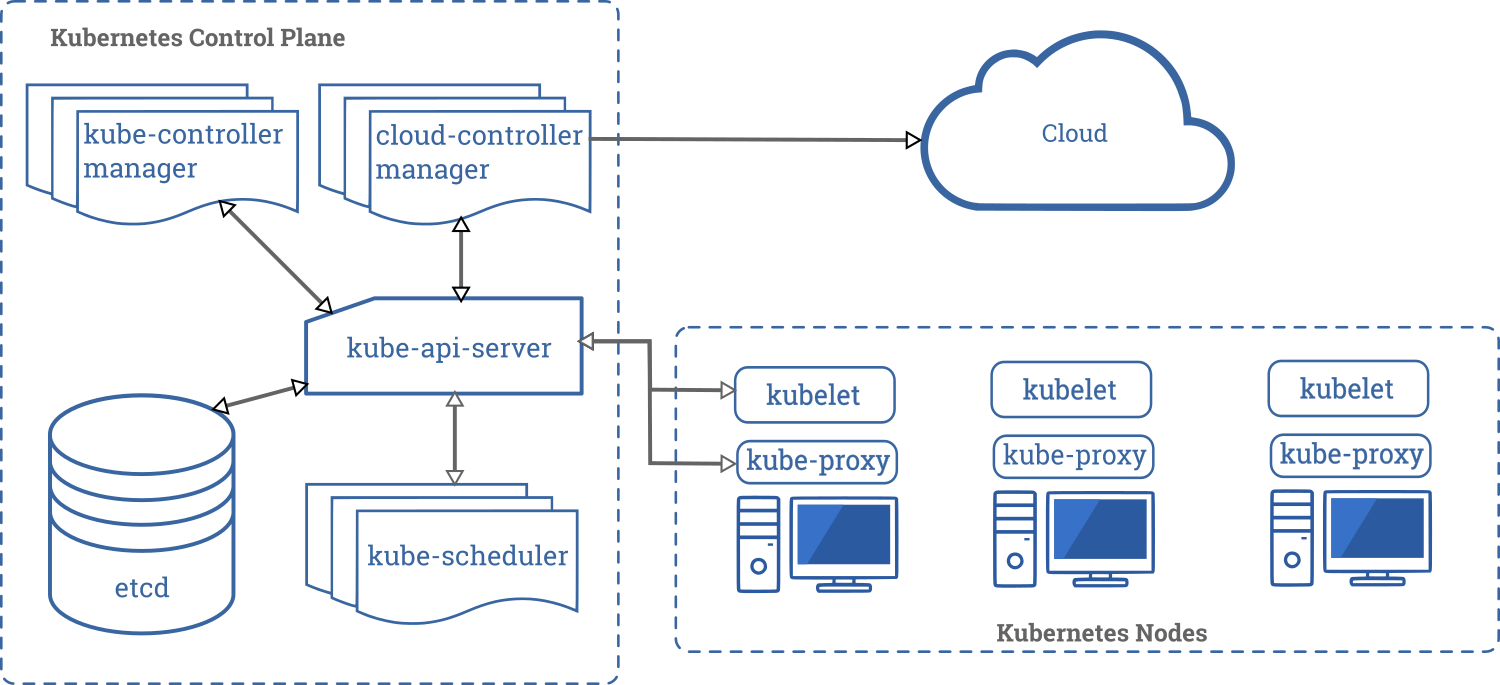
\includegraphics[width=1.0\textwidth]{./Figure/Kubernetes_Architettura.png}
 \caption{Architettura di Kubernetes}
 \label{fig:Architettura}
\end{figure}

\subsection{Kubernetes Control Plane}
Il Kubernetes Control Plane è il centro nevralgico delle operazioni del cluster. È costituito da una serie di componenti, in esecuzione all'interno del cluster, che hanno il compito di garantire l'integritá esecutiva del cluster, ad esempio, lo scheduling dei Worker Node e la gestione dei possibili failures dei Pod.
\begin{itemize}
    \item\textbf{kube-apiserver}
    kube-apiserver è il server API per il cluster Kubernetes. È il punto di contatto centrale a cui accedono tutti gli utenti, l'automazione e i componenti nel cluster Kubernetes. Il server API implementa un'API RESTful su HTTP, esegue tutte le operazioni API ed è responsabile dell'archiviazione degli oggetti API in un backend di archiviazione persistente. 
    \item\textbf{etcd}
    etcd è la componente di archiviazione principale di Kubernetes, etcd memorizza e replica tutti gli stati dei cluster Kubernetes. Il meccanismo di memorizzazione che adotta è di tipo chiave-valore ovvero ad ogni valore memorizzato viene associato una chiave che rappresenta il suo identificatore univoco. In questo modo il Control Plane è in grado di storicizzare gli stati del Cluster confrontando lo stato attuale con quello desiderato in modo di intervenire tempestivamente in caso di necessità.
    \item\textbf{kube-scheduler}
    kube-scheduler è la componente che consente al Control Plane lo scheduling dei Pod sui nodi. il kube-scheduler controlla i pod appena creati che non hanno un nodo assegnato, e dopo averlo identificato glielo assegna. 
    % DA RIVEDERE ✌️
    \item\textbf{kube-controller-manager} 
    Da un punto di vista logico, ogni controller è un processo separato, ma per ridurre la complessità, tutti i principali controller di Kubernetes vengono raggruppati in un unico container ed eseguiti in un singolo processo.
    Alcuni esempi di controller gestiti dal kube-controller-manager sono:
    Node Controller: Responsabile del monitoraggio dei nodi del cluster, e.g. della gestione delle azioni da eseguire quando un nodo diventa non disponibile.
    Replication Controller: Responsabile per il mantenimento del corretto numero di Pod per ogni ReplicaSet presente nel sistema
    Endpoints Controller: Popola gli oggetti Endpoints (cioè, mette in relazioni i Pods con i Services).
    Service Account e Token Controllers: Creano gli account di default e i token di accesso alle API per i nuovi namespaces.
    % DA RIVEDERE ✌️
    \item\textbf{cloud-controller-manager}
    Un componente della control plane di Kubernetes che aggiunge logiche di controllo specifiche per il cloud. Il cloud-controller-manager ti permette di collegare il tuo cluster con le API del cloud provider e separa le componenti che interagiscono con la piattaforma cloud dai componenti che interagiscono solamente col cluster.
    Il cloud-controller-manager esegue dei controller specifici del tuo cloud provider. Se hai una installazione Kubernetes on premises, o un ambiente di laboratorio nel tuo PC, il cluster non ha un cloud-controller-manager.
    Come nel kube-controller-manager, il cloud-controller-manager combina diversi control loop logicamente indipendenti in un singolo binario che puoi eseguire come un singolo processo. Tu puoi scalare orizzontalmente (eseguire più di una copia) per migliorare la responsività o per migliorare la tolleranza ai fallimenti.
    
    I seguenti controller hanno dipendenze verso implementazioni di specifici cloud provider:

    Node Controller: Per controllare se sul cloud provider i nodi che hanno smesso di rispondere sono stati cancellati
    Route Controller: Per configurare le network route nella sottostante infrastruttura cloud
    Service Controller: Per creare, aggiornare ed eliminare i load balancer del cloud provider

\end{itemize}


% %%%%%%%%%%%%%%%%%%%%%%%%%%%%
% \chapter{Stato dell'Arte}
% La crescente popolarità dell’approccio multi-cloud ha portato alla nascita di varie tecnologie che ne permettano l’utilizzo, ognuna delle quali utilizza un approccio specifico in base agli obiettivi che si pone. Inizialmente lo scopo degli strumenti era quello di fornire un modo per unificare la gestione e il controllo delle varie risorse fornite dai diversi provider, raggruppandole sotto un unico ambiente. È il caso di OpenStack \cite{OpenStack}, un software open-source rilasciato sotto licenza Apache che opera come un sistema operativo per Cloud. OpenStack permette di creare e gestire ambienti Cloud, sia pubblici che privati, attraverso risorse virtuali relative al modello IaaS, di conseguenza manca il supporto agli altri modelli, soprattutto al Serverless Computing. Un approccio simile è seguito da MODAClouds \cite{MODAClouds}, un framework che segue un approccio model-driven per la progettazione e l’esecuzione di applicazioni multi-cloud. Il punto di forza è il suo approccio model-driven che consente di progettare le applicazioni ad alto livello, in completa astrazione rispetto al Cloud di riferimento, e poterle eseguire su qualsiasi piattaforma. Il codice in questione viene infatti tradotto in base all’ambiente di esecuzione permettendo una facile integrazione di più servizi Cloud e rendendo particolarmente semplice la migrazione delle applicazioni da provider a provider. \\
Con l’avvento del Serverless Computing è nata la necessità di estendere gli strumenti esistenti per supportare questo modello. È il caso di TOSCA \cite{TOSCASite}, acronimo per
Topology and Orchestration Specification for Cloud Applications, un linguaggio di standard OASIS per la modellazione per lo sviluppo e la gestione di applicazioni su Cloud. In \citet{TOSCAServerless} viene esteso per integrare la possibilità di sfruttare le componenti Serverless all’interno delle applicazioni che si vuole creare. TOSCA permette di descrivere la struttura e il comportamento dei servizi forniti dal Cloud concentrandosi su portabilità e interoperabilità delle applicazioni descritte, risultando tuttavia mancante di alcune funzionalità critiche per le applicazioni Cloud in quanto non permette di specificare i requisiti di risorse. Un approccio molto simile è quello di CAMEL \cite{CAMELSite}, un Multi-Domain-Specific Language per la gestione del ciclo di vita delle applicazioni. Acronimo di Cloud Application Modelling and Execution Language, CAMEL consente di modellare componenti per applicazioni o servizi sfruttando più ambienti Cloud. Anche in questo caso il linguaggio viene esteso in \citet{@ServerlessCamel} che introduce un’estensione che supporti le componenti Serverless. CAMEL è un multi-DSL, l’unione di diversi DSL per coprire tutti gli aspetti del ciclo di vita di un’applicazione, ed è basato sulla tecnologia Xtext di Eclipse.
Basato su CAMEL MELODIC \cite{MELODIC} è un middleware che permette di automatizzare ed ottimizzare lo sviluppo di applicazioni multi-cloud. Tutte le componenti di MELODIC non sono legate ad un particolare Cloud provider ma possono essere utilizzate per qualsiasi ambiente su Cloud. L'integrazione all'interno di MELODIC del supporto alle componenti Serverless è descritto in \citet{ServerlessMultiCloud}. \\
Un altro tipo di soluzioni è quello dedicato esclusivamente alle componenti Serverless, di cui l’esponente maggiore è certamente Serverless \cite{ServerlessSite}, un framework web open-source scritto in Node.js. Serverless è il primo framework sviluppato per la costruzione di applicazioni basate sui servizi di Serverless Computing offerte dai principali Cloud provider, sono infatti supportati AWS Lambda di AWS, Azure Function di Microsoft Azure, IBM Bluemix e Google Cloud Platform. Serverless fornisce una CLI, Command Line Interface, per sviluppare le varie applicazioni fornendo esempi, strutture pre-costruite per agevolare il lavoro dello sviluppatore. Supportando tutti i maggiori Cloud provider, la Serverless Framework CLI fornisce un’esperienza di sviluppo singola per diversi provider. Punto a favore è la possibilità di testare le proprio applicazioni in locale, senza necessità di interagire con il provider, evitando quindi di incorrere in costi di esecuzione. Al contrario il limite di Serverless è proprio la specificità di servizio, dedicato alla costruzione di applicazioni puramente Serverless. \\
Un approccio diverso è proposto in \citet{DistributedFaas} in cui viene descritta un’architettura basata su container che permette di progettare e costruire un sistema distribuito tra diversi Cloud provider sul modello FaaS. Questa può essere vista come un’integrazione dei classici sistemi di High Performance Computing, formati da cluster di computer, declinati sul modello FaaS. Quello che si ottiene sono meccanismi di auto-scaling sia per macchine virtuali che per container in un ambiente distribuito multi-cloud, in aggiunta ad un sistema di bilanciamento del carico che tiene conto dei diversi cluster FaaS coinvolti. 


% %%%%%%%%%%%%%%%%%%%%%%%%%%%%
% \chapter{Fly Language}
% Implementare un’architettura multi-cloud non significa raggruppare semplicemente vari servizi di diversi Cloud provider in un unico sistema, ma richiede un approccio ragionato ben specifico. L'obiettivo è quello di creare un ambiente coeso che sfrutti in maniera efficace la collaborazione tra i diversi Cloud senza aumentare eccessivamente la complessità necessaria alla sua gestione. A causa della mancanza di standardizzazione, infatti, l'approccio multi-cloud richiede la conoscenza di diversi strumenti in quanto ogni Cloud provider fornisce le proprie API, metodi di accesso e protocolli di sicurezza rendendone difficile l’utilizzo. È facile comprendere come, se da una parte il multi-cloud può portare enormi vantaggi agli utenti che decidono di utilizzarlo, d’altro canto anche le difficoltà da affrontare non sono poche e c'è bisogno di soluzioni efficaci per superarli. \\
La chiave di volta nell’utilizzo del multi-cloud è sicuramente l’astrazione, ovvero l'utilizzo di strumenti che sollevano l'utente dalla necessità di conoscere tutti i dettagli implementativi per la gestione dell'ambiente, permettendo così di ottenere i vantaggi del multi-cloud evitando di introdurre complessità aggiuntiva \cite{ForbesMultiCloud}. Per venire incontro a questa esigenza nasce \textbf{Fly}, un \textbf{Domain-Specific Language} per il Calcolo Scientifico sul multi-cloud il cui obiettivo è quello di semplificare lo sviluppo di applicazioni che sfruttino la potenza computazionale offerta da molteplici Cloud provider, mediante il paradigma FaaS per ottenere alta scalabilità e alte prestazioni. Il punto di forza di Fly risiede nella gestione dell'interazione con il Cloud la quale viene completamente astratta all’utente finale che non necessita di conoscere le specifiche API del provider che vuole utilizzare \cite{ISISLab}. \\
L’aspetto innovativo di Fly è costituito dal concetto di \textbf{funzione Fly}, un blocco di codice indipendente che può essere eseguito in modo concorrente, in linea con il modello FaaS che utilizza funzioni Serverless. \\
Le caratteristiche principali di Fly sono potenza, efficacia ed efficienza:

\begin{itemize}
    \item Fly è \textit{potente} perché permette di sfruttare le capacità di computazione di diversi Cloud provider in una singola applicazione, utilizzando le soluzioni più efficienti in base alle necessità;

    \item Fly è \textit{efficace} perché è un linguaggio user-friendly, facile da comprendere ed utilizzare, che libera il programmatore dal dover gestire e configurare diversi ambienti di esecuzione;
    
    \item Fly è \textit{efficiente} perché permette di scegliere i servizi migliori sia dal punto di vista delle funzionalità che del costo, inoltre riduce i tempi di sviluppo grazie all'astrazione.
\end{itemize}

In questo capitolo saranno descritti i dettagli del linguaggio Fly, descrivendo gli obiettivi per cui è stato sviluppato, la sua architettura e il suo funzionamento. Viene inoltre introdotto il concetto di Domain-Specific Language e Xtext, il framework utilizzato per lo sviluppo di Fly.

\section{Obiettivi}
Fly nasce con lo scopo di riconciliare il Cloud Computing con l’High Performance Computing, fornendo uno strumento potente, semplice ed efficace per lo sviluppo di applicazioni Serverless di Calcolo Scientifico che sfruttino il sistema multi-cloud per ottenere un'alta scalabilità. \\
I principali obiettivi di Fly sono:

\begin{itemize}
    \item \textit{espressività} - possibilità di scrivere algoritmi con poche istruzioni, in modo chiaro e leggibile, in modo da rendere lo sviluppo di un programma di Calcolo Scientifico su larga scala semplice ed intuitivo anche per sviluppatori non esperti;
    
    \item \textit{alta usabilità} - scrivere un programma Fly deve essere semplice per gli esperti del dominio, l’interazione con l’ambiente Cloud deve essere completamente astratta eliminando la necessità di conoscere le API del Cloud provider;
    
    \item \textit{scalabilità} - sia architetture Symmetric Multiprocessing (SMP), sia architetture costruite su Cloud devono essere in grado di scalare facilmente.
\end{itemize}

Fly è stato progettato per permettere agli sviluppatori di dominio, ovvero esperti di un particolare campo con conoscenze limitate riguardo i complessi sistemi paralleli e distribuiti, di sviluppare le proprie applicazioni sfruttando il parallelismo mediante architetture Serverless. Infatti, la sintassi di Fly è ispirata a linguaggi come Java, JavaScript, Python e R, ovvero i più potenti e famosi linguaggi di programmazione utilizzati nel Calcolo Scientifico, in modo da proporre un ambiente familiare agli sviluppatori che lo utilizzano. Vengono forniti numerosi costrutti specifici per il dominio di interesse che vanno a formare un ricco linguaggio utilizzabile facilmente per interagire con i servizi su Cloud. \\
Fly supporta in modo implicito il paradigma di calcolo distribuito e parallelo insieme con la gestione della memoria fornendo inoltre un sistema di comunicazione di processi tramite appositi canali di comunicazione. Un programma Fly è infatti eseguibile sia su un'architettura multiprocessore sia su ambiente Cloud che supporti il modello FaaS, il tutto senza la necessità di conoscere in maniera precisa le risorse di computazione che occorrono per l'esecuzione \cite{ISISLab}.

\section{Domain-Specific Language}
Un \textbf{Domain-Specific Language (DSL)} è un linguaggio di programmazione progettato per essere utilizzato nel contesto di un particolare dominio, fornendo una notazione su misura basata sui concetti e le caratteristiche fondamentali per tale dominio. Un DSL rappresenta il concetto opposto rispetto ai linguaggi General Purpose che invece possono essere usati per un’ampia gamma di problemi e situazioni. Attraverso l’uso di un DSL viene introdotto un livello di astrazione che rende possibile anche ad esperti del dominio la creazione di soluzioni efficaci senza la necessità di avere competenze tecniche specifiche. Questo consente di affidare lo sviluppo di applicazioni software a figure che hanno una conoscenza del contesto più specifica invece che ai soli informatici, permettendo di incrementare l'efficacia e l'efficienza dell'intero processo.\\
Un DSL non ha lo scopo di essere utile a tutti, al contrario è creato per un risolvere problemi relativi ad un contesto molto specifico. Un esempio di linguaggi di questo tipo è HTML progettato per la costruzione di siti web e sicuramente non adatto alla creazione di applicazioni, ad esempio, di simulazione, dominio a cui è invece dedicato OpenABL. Altri DSL noti sono R per l’ambito statistico o SQL per la scrittura di query su database relazionali, il quale offre il vantaggio di non aver bisogno di essere un amministratore di database per scrivere semplici interrogazioni per l'ottenimento di dati. \\
Lo scopo principale di un DSL è quello di essere semplice da imparare e da utilizzare grazie proprio alla specificità di utilizzo che gli permette di essere piccolo, espressivo e poco ridondante, divenendo un punto d’incontro tra esperti del dominio e sviluppatori. \\
La realizzazione di un DSL passa per lo sviluppo di un compilatore che sia in grado di leggere il programma scritto in quel particolare linguaggio, analizzarlo, processarlo e interpretarlo per generare il codice eseguibile. Questo processo prevede una serie di fasi che sono descritte di seguito:

\begin{itemize}
    \item \textit{analisi lessicale} - il programma iniziale viene suddiviso in singole unità chiamate \textit{token}, ognuna delle quali corrisponde ad un singolo elemento del linguaggio;
    
    \item \textit{analisi sintattica} - i \textit{token} identificati vengono analizzati per assicurarsi che formino uno statement valido per il linguaggio. È in questa fase che viene prodotto l’Abstract Syntax Tree (ABS), ovvero la rappresentazione della struttura sintattica del programma;
    
    \item \textit{analisi semantica} - comprende la fase di type checking che controlla che gli assegnamenti di valore siano compatibili con il relativo tipo di dati insieme con la fase di tracciamento degli identificatori, del loro tipo e delle espressioni che si assicura anche che i primi siano stati dichiarati prima dell’uso;
    
    \item \textit{generazione del codice} - parte finale che utilizza i risultati delle fasi precedenti per generare il codice macchina o, eventualmente, il programma scritto in un altro linguaggio.
\end{itemize}

\subsubsection{Xtext}
\textbf{Xtext} \cite{Xtext} è un framework open-source per lo sviluppo di linguaggi di programmazione e DSL. Diversamente dai comuni strumenti disponibili, Xtext genera non solo un parser ma anche un class model per l’Abstract Syntax Tree, fornendo anche un IDE, ovvero un ambiente di sviluppo, basato su Eclipse completo di tutte le funzioni e personalizzabile. Lo sviluppo di un linguaggio attraverso Xtext si basa sulla scrittura di una grammatica che lo definisce in tutte le sue parti, essa permette di ottenere un’infrastruttura completa inclusa di parser, linker, typechecker e compilatore insieme con il supporto all’editing per Eclipse. L’utilizzo di un framework come Xtext offre enormi vantaggi agli sviluppatori di DSL ed è per questo motivo che è stato scelto per la creazione del compilatore source-to-source di Fly.

\section{Architettura}
Utilizzare Fly per implementare la propria applicazione permette all'utente di non preoccuparsi della quantità di risorse necessaria all'esecuzione, in quanto esse vengono stabilite in automatico in base ai requisiti di computazione. Sono supportati modelli di esecuzione sia sincroni che asincroni ed è possibile scegliere tra due ambienti di run-time, ovvero la macchina locale o l'infrastruttura Cloud. Quest'ultima viene considerata come un'architettura di calcolo parallelo utilizzabile per l'esecuzione di codice concorrente grazie a costrutti specifici atti a facilitare l'esperienza dell'utente. \\
Fly risulta in un linguaggio staticamente e fortemente tipizzato che sfrutta varie tipologie di inferenza per determinare il tipo delle variabili e delle costanti dichiarate. Un programma scritto in Fly viene tradotto in automatico dal compilatore in codice Java, nello specifico ogni tipo di dato presente all'interno di Fly ha un suo corrispettivo in quest'ultimo linguaggio, così come le varie funzionalità specifiche del dominio vengono realizzate sfruttando l'ampia gamma di metodi offerti dal linguaggio General Purpose. \\
L’elemento fondamentale di Fly è rappresentato dal concetto di \textbf{funzione Fly}, ovvero una porzione di codice indipendente che eseguita in maniera concorrente, similmente a quanto avviene con le funzioni Serverless del modello FaaS. Le funzioni Fly possono essere eseguite in sequenziale o in parallelo, sia su infrastruttura locale multi-processore che su Cloud mediante l'utilizzo di appositi costrutti che ne permette la definizione, l'esecuzione, la sincronizzazione e la gestione della comunicazione. Quest’ultima viene resa disponibile anche tra processi differenti in esecuzione su diversi ambienti attraverso l'uso di appositi canali di comunicazione virtuali i quali rappresentano il metodo principale per lo scambio di dati tra diverse funzioni Fly. \\ 

\begin{figure}[htbp]
 \centering
 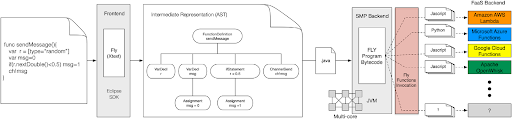
\includegraphics[scale=0.7]{./Figure/FLYCompilazione.png}
 \caption{Flusso di compilazione di Fly.}
 \label{fig:compilazione}
\end{figure}

La \figurename~\ref{fig:compilazione} mostra il \textbf{flusso di una compilazione} in Fly. Partendo da sinistra il programma Fly viene fornito in input al compilatore che genera un \textit{Abstract Syntax Tree (AST)}, ovvero un albero rappresentante la struttura sintattica del codice in cui ogni costrutto corrisponde ad un nodo. Viene definito astratto in quanto non vengono rappresentati tutti i dettagli del codice sorgente ma solo la sua struttura. In seguito la rappresentazione in AST intermedia viene trasformata in un programma Java da cui vengono estratte le singole funzioni Fly, ognuna delle quali verrà tradotta in diversi codici eseguibili, uno per ogni ambiente dichiarato dall’utente. Infine, osservando il lato destro della \figurename~\ref{fig:compilazione} è possibile osservare l’output finale che consiste nel codice compilato delle funzioni Fly pronto per essere eseguito sui vari ambienti dichiarati.

\begin{figure}[htbp]
 \centering
 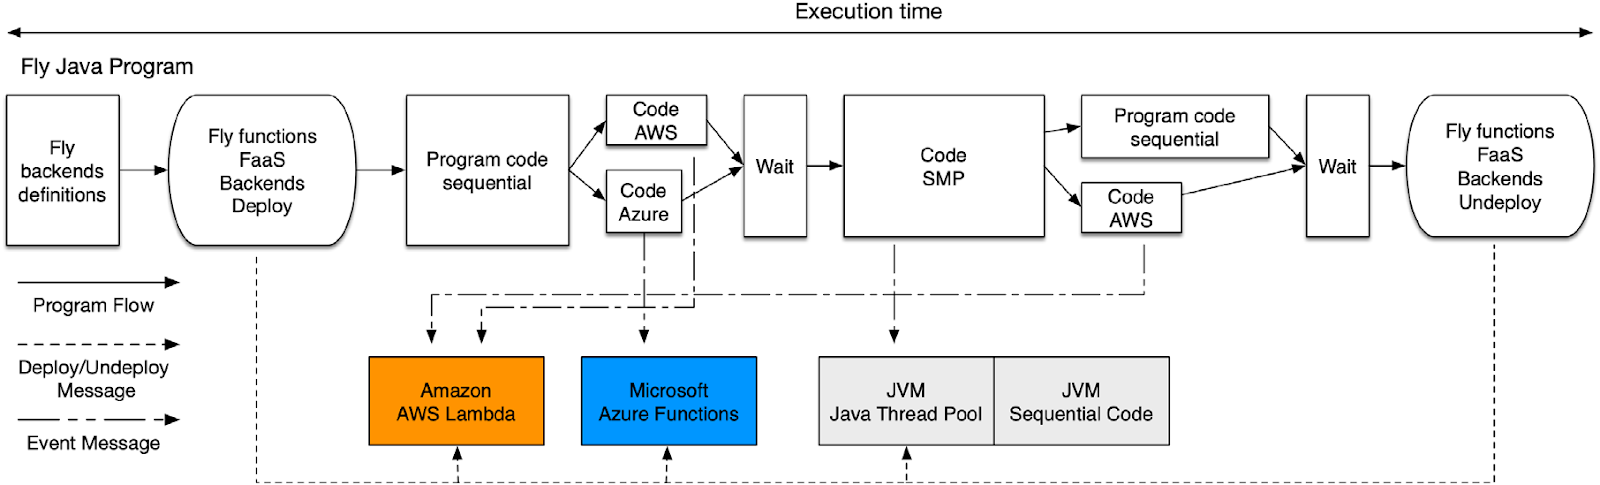
\includegraphics[scale=0.22]{./Figure/FLYEsecuzione.png}
 \caption{Flusso di esecuzione di Fly.}
 \label{fig:esecuzione}
\end{figure}

Nella \figurename~\ref{fig:esecuzione} viene mostrato nel dettaglio il flusso di esecuzione che inizia al lancio di un programma Fly. Seguendo il tempo di esecuzione, la prima fase prevede l’inizializzazione degli ambienti di back-end dichiarati all’interno del codice, questa prevede il login sul Cloud provider e l’istanziazione dei servizi necessari. Il codice generato a partire dalla funzione Fly viene poi caricato sul rispettivo ambiente Cloud, esso risulterà già compilato nel momento in cui il programma principale viene lanciato, in questo modo si evitano i tempi di attesa che sarebbero causati da una compilazione a tempo di esecuzione. Effettuata la fase di inizializzazione il programma principale viene mandato in esecuzione seguendo le istruzioni contenute nel codice Fly e al suo termine vengono effettuate una serie di procedure di undeploy sull’ambiente di back-end, avente lo scopo di eliminare tutte le istanze dei servizi Cloud creati in precedenza.

\section{Definizione del linguaggio}
Fly fornisce diversi tipi di dati che possono essere raggruppati in due insiemi, \textit{basici} e di \textit{dominio}. I primi sono ereditati da Java e comprendono \textit{booleani}, \textit{interi}, \textit{reali} e \textit{stringhe}, essi possono essere usati anche per la dichiarazione di array monodimensionali, bidimensionali e tridimensionali. Di numero maggiore sono invece i tipi di dominio utilizzabili in Fly che permettono all'utente di interagire e comunicare con l'ambiente di esecuzione.\\
Il Listato~\ref{lst:pigreco} mostra un semplice esempio di programma Fly per il calcolo di una stima di Pi Greco tramite il metodo Monte Carlo su ambiente Amazon Web Services, in particolare sfruttando il servizio AWS Lambda \cite{LambdaSite}. È utile fornire una prima descrizione del codice i cui elementi verranno poi approfonditi in seguito. Alla Riga 1 troviamo la dichiarazione dell'ambiente di esecuzione, in questo caso viene definito su AWS. Su tale ambiente è dichiarato un \verb|channel|, Riga 3, che permette al programma principale di comunicare con la funzione Fly \verb|hit| definita alla Riga 5, la quale genera un punto casuale e calcola se appartiene o meno ad un cerchio che abbia origine al punto 1.0, realizzando l'algoritmo per il metodo Monte Carlo. Il valore ottenuto viene poi inviata sul canale \verb|ch|. La funzione \verb|estimation|, Linea 16, legge l'output della funzione \verb|hit| e scrive a schermo la stima di Pi ottenuta. Alla linea 28 è possibile vedere come sono lanciate le funzioni Fly, in particolare viene utilizzata la parola chiave \verb|fly| per eseguire 10000 funzioni \verb|hit| sull'ambiente AWS. Infine l'utilizzo della parola chiave \verb|thenall| fa in modo che quando tutte le funzioni \verb|hit| hanno terminato venga eseguita la funzione \verb|estimation|.\\

\begin{lstlisting}[language=FLY,caption={Stima di PI Greco usando il metodo Monte Carlo su ambiente AWS.}, label={lst:pigreco}]
var local = [type="smp", nthread=4]

var cloud = [type="aws", user="user_name", access_id_key = "access_id_key", secret_access_key="secret_access_key", region="eu-west-2", language="nodejs12.x", thread=2, memory=256, time_=300]

var ch = [type="channel"] on cloud

func hit(){	
    var r = [type="random"]
    var x = r.nextDouble()
    var y = r.nextDouble()
    var msg = 0
    
    if((x * x)+(y * y) < 1.0){msg = 1}
    ch!msg on cloud
}


func estimation(){
    var sum = 0
    var crt = 0
    for i in [0:2] {
        sum += ch? as Integer
        crt += 1
    }
    println "pi estimation: " + (sum*4.0) \ crt
}

fly hit in [0:2] on cloud thenall estimation  
\end{lstlisting}  

\subsubsection{Object} 
Il principale tipo di dato di dominio è il tipo \verb|object|, un insieme eterogeneo di elementi di tipo basico e/o di dominio. Un Fly \verb|object| può essere visto come l'unione di un \verb|array|, un classico vettore, e di una \verb|mappa|, ovvero una struttura dati in grado di memorizzare elementi nella forma di coppie chiave-valore. Il valore di un elemento può essere ottenuto in due diversi modi, utilizzando la sua posizione, come si fa per gli array, o la sua chiave, come nel caso di una mappa. Quando un nuovo valore è assegnato ad una data chiave o posizione viene creato un nuove elemento, altrimenti il nuovo valore va a sostituire il precedente. \\
Ogni tipo di dato di dominio presente in Fly è un'istanza del tipo \verb|object|, questo fa sì che essi siano costruiti tutti con una sintassi simile utilizzando il campo \verb|type| per specificarne il tipo.

\subsubsection{Ambiente di esecuzione}
Il codice di un programma Fly inizia sempre con la dichiarazione di uno o più \textbf{ambienti di esecuzione}, necessari affinché il generatore possa configurare le risorse utili al funzionamento dell'applicazione, in particolare è sempre necessario un ambiente di esecuzione locale corrispondente alla macchina su cui viene lanciato il programma. Ad esempio nel caso di un ambiente locale multiprocessore viene utilizzata una \verb|Java Thread Pool| mentre per gli ambienti su Cloud è necessario creare le istanze dei servizi necessari. Il grande vantaggio offerto da Fly è l'astrazione, dal punto di vista dello sviluppatore infatti tutti i tipi di ambienti possono essere utilizzati allo stesso modo, sarà il compilatore ad occuparsi dei dettagli implementativi specifici relativi al loro utilizzo. \\
La dichiarazione di un ambiente di esecuzione necessita di una serie di parametri che variano in base alla tipologia di ambiente, specificata dal campo \verb|type|. Oltre ad eventuali informazioni aggiuntive richieste dai diversi Cloud provider per accedere ai loro servizi, la dichiarazione relativa ad un'esecuzione su Cloud richiede che l'utente specifichi il linguaggio di programmazione in cui verranno tradotte le funzioni Fly per essere lanciate sul servizio Serverless del provider. In particolare le possibilità sono JavaScript \cite{JavaScriptSite} o Python \cite{PythonSite}.\\
Attualmente gli ambienti supportati sono tre, quattro con l'implementazione trattata in questo lavoro di tesi (vedi Capitolo~\ref{debug}):

\begin{itemize}
    \item \textbf{smp} - ambiente locale che sfrutta il parallelismo basato su un sistema multiprocessore simmetrico sfruttando i thread Java;
    
    \item \textbf{aws} - ambiente su Cloud legato al provider Amazon Web Services (AWS)  \cite{AmazonSite} che sfrutta il servizio AWS Lambda \cite{LambdaSite} per eseguire le funzioni Fly;
    
    \item \textbf{azure} - ambiente su Cloud legato al provider Microsoft Azure \cite{MicrosoftSite} che sfrutta il servizio Azure Function \cite{FunctionSite} per eseguire le funzioni Fly. In questo caso il supporto a Python non è previsto in quanto al momento dell'implementazione non ancora reso disponibile da Azure.
\end{itemize}

\subsubsection{Channel}
La comunicazione e la sincronizzazione sia tra le varie funzioni Fly, sia tra queste e il programma principale avviene mediante la dichiarazione di un \verb|type|\verb|=|\verb|"channel"| che necessita di specificare l'ambiente di esecuzione sul quale funzionare mediante la parola chiave \verb|on|. Questo metodo di comunicazione segue il modello delle code di messaggi bloccanti, ovvero quando si tenta di ricevere un messaggio l'esecuzione si ferma fino a che un nuovo messaggio non viene ricevuto. L'utilizzo del carattere \verb|"!"| permette l'invio di messaggi, vedi Riga 13 del Listato~\ref{lst:pigreco}, mentre il carattere \verb|"?"| è necessario per la loro ricezione, vedi Riga 22 del Listato~\ref{lst:pigreco}. Fly implementa un meccanismo di serializzazione in quando la comunicazione utilizza le infrastrutture di rete per scambiare messaggi con l'ambiente su Cloud.

\subsubsection{Funzione Fly}
Le \textbf{funzioni Fly} sono già state in parte descritte, esse sono frammenti di codice scritto per realizzare una funzionalità specifica indipendente dal programma principale e da altre funzioni ed eseguibile in maniera concorrente. Queste funzioni sono ben diverse da quelle disponibili in altri linguaggi di programmazione e prendono ispirazione da quelle utilizzate nei linguaggi funzionali.\\
La dichiarazione di una funzione Fly è possibile utilizzando la parola chiave \verb|func| a seguito della quale si definisce il nome della funzione e si inseriscono eventuali parametri di input tra parentesi che vengono passati per copia e sono considerati immutabili. Le funzioni Fly possono restituire un valore mediante l'uso della parola chiave \verb|return| ed hanno scoping privato, ovvero solo i parametri della funzione e le variabili locali sono visibili all'interno del corpo della funzione. Per superare tale limitazione possono essere utilizzati sia gli oggetti \verb|channel| che le costanti a patto che la dichiarazione e l'accesso avvengano nello stesso ambiente di esecuzione. Questo significa che se una funzione è in esecuzione sull'ambiente X essa può utilizzare canali e oggetti disponibili su tale ambiente X a prescindere da chi li abbia dichiarati.
Le funzioni Fly possono essere eseguite in modo concorrente utilizzando la parola chiave \verb|fly|, non essendo ammessa la ricorsione essa non può essere utilizzata all'interno del corpo di una funzione. Il suo utilizzo causa la generazione di un evento sull’ambiente che si sta utilizzando, sia esso SMP o su Cloud, in modo che le funzioni vengano eseguite, in linea con il modello di programmazione event-driven che caratterizza il Serverless Computing. Il parallelismo esplicito da cui è caratterizzato Fly è racchiuso nel modo in cui vengono lanciate le funzioni, a seguito della parola chiave \verb|fly| viene dichiarata il nome della funzione da eseguire e, se necessario, il loro numero insieme alla variabile che rappresenta l'ambiente di esecuzione da utilizzare specificato in seguito alla parola chiave \verb|on|.

\subsubsection{Funzione di Callback}
Le \textbf{funzioni di Callback} sono funzioni Fly che vengono eseguite al termine dell'esecuzione di una precedente funzione. Esse possono essere dichiarate dopo la specifica dell'ambiente di esecuzione su cui deve essere eseguita una funzione Fly. Due tipi di funzioni di Callback sono supportate, la prima riguarda quelle specificate in seguito alla parola chiave \verb|then| che indica che la sua esecuzione deve avvenire dopo ogni singola funzione Fly, mentre utilizzando la parola chiave \verb|thenall| si richiede che la funzione venga eseguita solamente quando tutte le funzioni Fly hanno terminato.

\subsubsection{Esecuzioni asincrone}
Fly permette \textbf{esecuzioni asincrone} attraverso l'uso della parola chiave \verb|async| e tipo di dato di dominio chiamato \verb|async-object| che permette all'utente di controllare ed interagire esse. Invocando una funzione utilizzando \verb|async| viene restituito immediatamente il controllo al programma principale in modo che l'esecuzione possa continuare, a questo punto l'utente può controllare lo stato delle funzioni asincrone usando il metodo \verb|status()| dell'\verb|async-object|, mentre il metodo \verb|wait()| mette in pausa l'esecuzione fino a che tutte le funzioni non hanno terminato.

\subsubsection{Codice nativo}
La possibilità di includere \textbf{codice nativo} all'interno di applicazioni Fly è data dalla parola chiave \verb|native|, tale funzionalità consente, ad esempio, di inserire in una funzione Fly codice scritto direttamente in Python ed esso non verrà tradotto o modificato dal compilatore Fly ma copiato così com'è. Tramite la parola chiave \verb|require| è inoltre consentito includere ed installare librerie esterne addizionali nell'ambiente di esecuzione.

\subsection{Struttura di un progetto Fly}
Fly utilizza il gestore di pacchetti \textit{Maven} \cite{MavenSite} per la costruzione e la generazione dei progetti. Maven è uno strumento per la gestione di progetti software e di build automation basato sul concetto di \textbf{Project Object Model (POM)}, un file XML che contiene le dipendenze necessarie al funzionamento dell'applicazione. \\
La creazione di un \textbf{progetto Fly} genera due cartelle principali insieme con un file POM, il tutto racchiuso in un progetto Java Maven che include tutte le dipendenze, il programma principale e il codice delle funzioni, il tutto costruito sulla base del programma Fly da parte del compilatore. Attraverso il comando \verb|mvn package| di Maven tale progetto viene utilizzato per la generazione del file \textit{JAR} eseguibile \cite{ISISLab}.\\
Un progetto Fly è così strutturato:

\begin{itemize}
    \item \textbf{cartella \textit{src}} - cartella in cui è posizionato il file con estensione \textit{.fly} contenente il codice del programma scritto in linguaggio Fly;
    
    \item \textbf{cartella \textit{src-gen}} - cartella contenente i file generati dal compilatore che consistono in un file Java e due file di script. Il file Java ha il compito di orchestrare l'intera esecuzione del programma, ovvero l'intero ciclo di vita comprensivo del lancio dei due file di script. Questi ultimi sono file con estensione \textit{.sh} e contengono distintamente i comandi per il deploy delle funzioni Fly e le procedure per l'undeploy. Il file di deploy si occupa di creare il file necessario alla creazione della funzione Serverless sul servizio FaaS del provider definito, comprensivo di codice, librerie e file di configurazione, mentre il file di undeploy ha il compito di ripulire l'ambiente Cloud dalle risorse create;
    
    \item \textbf{file XML \textit{pom.xml}} - unità fondamentale di Maven per la gestione del progetto, si tratta di un file XML che contiene informazioni e i dettagli di configurazione necessari per effettuare la build, nel caso specifico al suo interno sono presenti le librerie necessarie al programma \cite{MavenPom}.
\end{itemize}

\section{Generazione del codice}
Il punto di forza di Fly è quello di fornire un livello di astrazione tale per cui l'utente non deve conoscere le API di ogni Cloud provider per scrivere un programma che sfrutti al meglio i suoi servizi. Tali API restano comunque essenziali per interagire con essi, infatti è il compilatore di Fly che si occupa di prendere in input il programma per tradurlo in codice effettivamente eseguibile. È quello che avviene nella fase di generazione del codice in cui ogni componente scritta in linguaggio Fly viene trasformata nel linguaggio di destinazione, il quale varia a seconda del contesto, come visto nei paragrafi precedenti. Possiamo quindi affermare che il fulcro del compilatore di Fly è sicuramente la parte di generazione di codice che produce un programma diverso in base all’ambiente di esecuzione dichiarato dall’utente. Nel caso di un ambiente multiprocessore il parallelismo viene implementato attraverso l’uso di una \verb|Java Thread Pool| che permette l'utilizzo di thread ai quali viene assegnata una specifica esecuzione, in particolare essa permette di riutilizzare thread precedentemente creati, eliminando il tempo necessario alla loro creazione. Il programma Fly viene quindi eseguito su una \textit{Java Virtual Machine (JVM)} come un classico programma Java, sulla quale viene eseguito anche l’ambiente SMP, assumendo quindi che siano disponibili almeno due core fisici, uno per l’esecuzione del programma e uno per l’ambiente. L'esecuzione su Cloud prevede invece l'utilizzo delle API fornite dal provider di riferimento che consentono di interagire con i servizi disponibili in base ai quali vengono tradotti i vari costrutti e funzionalità di Fly.\\
Il codice generato per le funzioni Fly varia in base all'ambiente di esecuzione scelto, in particolare il linguaggio di destinazione può essere Java, JavaScript o Python in base a quanto specificato dall'utente. In caso di esecuzione su ambiente SMP locale le funzioni sono tradotte in Java, in quanto eseguite su JVM, diversamente dal Cloud i cui servizi FaaS permettono solitamente l'esecuzione di codice in JavaScript o Python. Oltre al linguaggio utilizzato, l’ambiente di destinazione determina anche il modo in cui viene generato lo script di deploy che costruisce il pacchetto di esecuzione contenente codice sorgente e librerie. \\
Durante la fase di esecuzione l'interazione con il Cloud avviene mediante l'utilizzo degli strumenti di \textbf{Command Line Interface} forniti dai vari provider come la \textit{AWS CLI} \cite{awsCLI} o la \textit{Azure CLI} \cite{azureCLI}, mentre le funzioni vengono invocate con delle chiamate \textit{HTTP POST} asincrone, le quali assicurano la minor latenza permettendo al programma di continuare la sua esecuzione in attesa di risposta da parte del servizio.

\subsubsection{Amazon Web Services}
Amazon Web Services mette a disposizione diverse SDK che permettono di interagire con i suoi servizi praticamente con tutti i principali linguaggi di programmazione \cite{awsSDK}. Il programma principale, essendo scritto in Java fa uso delle \textit{AWS SDK for Java} \cite{AwsJavaSDK} che consentono di accedere a tutti i servizi forniti da AWS mediante delle API dedicate. Gli script di deploy e undeploy invece utilizzano la AWS CLI \cite{awsCLI} per creare le istanze di servizi necessarie al funzionamento del programma e per caricare le funzioni Fly e i relativi pacchetti su AWS Lambda. Queste ultime sfruttano la libreria \textit{boto3} per Python \cite{AwsPySDK} e la libreria \textit{aws-sdk} per JavaScript \cite{AwsJsSDK} per interagire con i servizi di AWS.

\subsubsection{Microsoft Azure}
Le SDK di Microsoft Azure soffrono di alcune problematiche di utilizzo derivanti sia dalla difficile integrazione al di fuori dell’IDE VisualStudio Code, sia dalla mancanza di funzionalità per gran parte dei servizi. Per questo motivo il supporto ad Azure passa per l’utilizzo di un servizio REST API che prescinde dal linguaggio di programmazione in quanto basato su operazioni HTML. Le \textit{Representational State Transfer (REST) API} consistono in endpoint specifici per ogni servizio che supportano un insieme di operazioni HTTP i quali forniscono l’accesso alle principali funzionalità di un servizio come la creazione, l’aggiornamento, la cancellazione o l’ottenimento di informazioni. L’utilizzo delle REST API è regolato dall’utilizzo di un token di autorizzazione ottenibile tramite il servizio Azure Active Directory che ne permette l’acquisizione fornendo i propri dati di accesso, in particolare ID, password e TenantID.
\newpage 
Le sezione seguenti analizzano come il codice scritto in Fly viene tradotto dal compilatore nei vari linguaggi di destinazione per generare i file eseguibili. Tutti i Listati mostrati fanno riferimento al programma  per il calcolo di Pi Greco, proposto nella sua interezza nel Listato~\ref{lst:pigreco}.

\subsection{Ambiente di esecuzione}

\subsubsection{Ambiente locale - SMP}
La dichiarazione di un \textbf{ambiente locale} necessita di due parametri, il primo definisce il tipo di ambiente che sarà di \verb|type|\verb|=|\verb|"smp"|, il secondo specifica il numero di thread che dovranno essere utilizzati.\\

\begin{lstlisting}[language=FLY,caption={Dichiarazione di un ambiente di esecuzione locale.}, label={lst:smp}]
var local = [type = "smp", nthread = 4]
\end{lstlisting}

Il codice Java generato risulta in un oggetto \verb|ExecutorService| che semplifica l'esecuzione asincrona, permettendo di eseguire i task in modo concorrente. Esso fornisce automaticamente un insieme di thread con una serie di metodi che permettono di assegnare loro dei task.\\

\begin{lstlisting}[language=Java,caption={Codice generato per l'ambiente di esecuzione locale.}, label={lst:localJava}]
static ExecutorService __thread_pool_local = Executors.newFixedThreadPool(4);
\end{lstlisting}

\subsubsection{Ambiente su Cloud - Amazon Web Services}
L'utilizzo di un ambiente di esecuzione che utilizzi il \textbf{Cloud AWS} è possibile mediante la dichiarazione di una variabile di \verb|type|\verb|=|\verb|"aws"| la quale necessita di una serie di parametri corrispondenti alle caratteristiche necessarie al lancio delle funzioni Serverless su AWS Lambda \cite{LambdaConfiguration}:

\begin{itemize}
    \item \textbf{dati di accesso dell'account AWS}: in ordine sono necessari \verb|user_name|, \verb| access_id_key|, \verb|secret_access_key|;
    \item \textbf{regione}: id della regione su cui si vogliono lanciare i servizi;
    \item \textbf{linguaggio}: linguaggio di programmazione in cui verranno tradotte ed eseguite le funzioni Lambda. Può essere \verb|nodejs| per JavaScript o \verb|python| per Python;
    \item \textbf{thread}: numero di istanze concorrenti da lanciare per l'esecuzione delle funzioni;
    \item \textbf{memoria}: quantità di memoria disponibile per l'esecuzione di una funzione;
    \item \textbf{time}: tempo limite di esecuzione per ogni funzione.
\end{itemize}



\begin{lstlisting}[language=FLY,caption={Dichiarazione di un ambiente Cloud su AWS.}, label={lst:aws}]
var cloud = [type="aws", user="user_name", access_id_key = "access_id_key", secret_access_key="secret_access_key", region="eu-west-2", language="nodejs12.x", thread=2, memory=256, time_=300]
\end{lstlisting}

Nel Listato~\ref{lst:awsJava} vediamo come vengono istanziati i servizi necessari all'esecuzione di un programma Fly utilizzando le informazioni fornite nella dichiarazione dell'ambiente. Tra i servizi troviamo AWS SQS \cite{SQS} per le code di messaggi, AWS IAM \cite{IAM} per l'autenticazione, AWS S3 \cite{S3} per la memorizzazione di dati e AWS Lambda \cite{LambdaSite} per l'esecuzione di funzioni Serverless.\\

\begin{lstlisting}[language=Java,caption={Codice generato per l'ambiente Cloud su AWS.}, label={lst:awsJava}]
static BasicAWSCredentials cloud = new BasicAWSCredentials("access_id_key", "secret_access_key");
		
static AmazonSQS __sqs_cloud  = AmazonSQSClient.builder()
	.withCredentials(new AWSStaticCredentialsProvider(cloud))
	.withRegion("eu-west-2")
	.build();
		
static AmazonIdentityManagement __iam_cloud = AmazonIdentityManagementClientBuilder.standard()
	.withCredentials(new AWSStaticCredentialsProvider(cloud))
	.withRegion("eu-west-2")
	.build();
			
static AWSLambda __lambda_cloud = AWSLambdaClientBuilder.standard()
	.withCredentials(new AWSStaticCredentialsProvider(cloud))
	.withRegion("eu-west-2")
	.build();
			
static AmazonS3 __s3_cloud = AmazonS3Client.builder()
    .withCredentials(new AWSStaticCredentialsProvider(cloud))
    .withRegion("eu-west-2")
    .build();
\end{lstlisting}

\subsubsection{Ambiente su Cloud - Microsoft Azure}
Utilizzare i servizi a disposizione sul \textbf{Cloud di Microsoft Azure} mediante linguaggi di programmazione risulta complesso e macchinoso a causa delle SDK fornite che, attualmente, presentano molteplici mancanze oltre ad una documentazione particolarmente scarna e spesso non aggiornata. Per tale motivo si è scelto di utilizzare il sistema di REST API attraverso delle chiamate \textit{HTTP}. L'integrazione dei servizi di Microsoft Azure all'interno del codice Java generato dal compilatore Fly è resa possibile grazie alla libreria AzureClient sviluppata presso l'ISISLab \cite{Grieco}, la quale permette di superare il problema della frammentazione delle SDK fornendo un'unica interfaccia che permette un più agevole utilizzo dei servizi. La gestione dei servizi di Azure con JavaScript soffre dei medesimi problemi in termini di SDK ed anche in questo caso è necessario utilizzare delle chiamate \textit{HTTP} per utilizzarli, in particolare vengono utilizzate le librerie \textit{axios} \cite{axios} e \textit{qs} \cite{qs}. In entrambi i casi rimane indispensabile il servizio Azure AD \cite{azureAD} per ottenere il \textit{token} di autorizzazione che permette di effettuare tali chiamate.\\
L'utilizzo di un ambiente di esecuzione che utilizzi il \textbf{Cloud Azure} è possibile mediante la dichiarazione di una variabile di \verb|type|\verb|=|\verb|"azure"| la quale necessita di una serie di parametri corrispondenti alle caratteristiche necessarie al lancio delle funzioni Serverless sul servizio Azure Function \cite{azureFunction}:

\begin{itemize}
    \item \textbf{dati di accesso dell'account Azure}: in ordine sono necessari \verb|client_id|,  \verb|tenant_id|, \verb|secret_key|, \verb|subscription_id|;
    \item \textbf{regione}: id della regione su cui si vogliono lanciare i servizi;
    \item \textbf{linguaggio}: linguaggio di programmazione in cui verranno tradotte ed eseguite le funzioni Lambda. Può essere \verb|nodejs| per JavaScript o \verb|python| per Python;
    \item \textbf{thread}: numero di istanze concorrenti da lanciare per l'esecuzione delle funzioni;
    \item \textbf{time}: tempo limite di esecuzione per ogni funzione.
\end{itemize}



\begin{lstlisting}[language=Java,caption={Dichiarazione di un ambiente Cloud su Azure.}, label={lst:azure}]
var cloud = [type="azure", clientID="client_id", tenantID="tenant_id", secret_key="secret_key", subscriptionID="subscription_id", region="France Central", language="nodejs12.x", threads="2", seconds="300"]
\end{lstlisting}

Il codice generato, visibile nel Listato~\ref{lst:azureJava}, comprende la creazione di una variabile istanza della libreria AzureClient necessaria per avviare tutte le procedure relative ai servizi di Azure. In particolare il metodo \verb|init()| si occupa di istanziare tutti i servizi di base indispensabili per l'esecuzione di qualsiasi programma Fly, sfruttando le informazioni fornite nella dichiarazione dell'ambiente per effettuare l'accesso al Cloud. Il metodo \verb|createFunctionApp(...)| invece è adibito alla creazione dell'istanza del servizio Serverless di Azure che permette l'esecuzione delle funzioni.\\

\begin{lstlisting}[language=Java,caption={Codice generato per l'ambiente Cloud su Azure.}, label={lst:azureJava}]
cloud = new AzureClient("client_id",
    "tenant_id",
    "secret_key",
    "subscription_id",
    __id_execution+"",
    "France Central");
    
cloud.init();

cloud.createFunctionApp("flyappcloud","nodejs12.x");
\end{lstlisting}

\subsection{\textit{Channel}}
La dichiarazione di un \verb|type|\verb|=|\verb|"channel"|, ovvero il mezzo di comunicazione e sincronizzazione utilizzato da Fly, necessita come unica specifica l'ambiente di esecuzione su cui dovrà funzionare, come mostrato nel Listato~\ref{lst:flyChannel}. Questo viene specificato mediante la parola chiave \verb|on| e in base ad esso il compilatore genererà un codice differente, adattandolo in modo che sfrutti i servizi di gestione delle code forniti dall'ambiente specificato. In particolare per AWS si utilizza il servizio AWS Simple Queue Service (SQS) \cite{SQS} mentre per Azure si sfruttano i metodi presenti all'interno della libreria AzureClient.\\
La logica di funzionamento dei prevede che ad uno dei thread dell'ambiente locale venga associato il task di lettura della coda rimanendo costantemente in ascolto e non appena vengono intercettati dei messaggi essi vengono immediatamente scritti sul canale sul quale è possibile leggerli.\\

\begin{lstlisting}[language=Java,caption={Dichiarazione di un \textit{Channel} su Cloud.}, label={lst:flyChannel}]
var ch = [type="channel"] on cloud
\end{lstlisting}

\subsection{Script di deploy e undeploy delle funzioni}
Il funzionamento delle funzioni Serverless su un ambiente Cloud richiede una serie di procedure sia per il deploy che per l'undeploy che vengono eseguite mediante gli strumenti di Command Line Interface forniti dai provider, di conseguenza i comandi cambiano in base al Cloud ma al linguaggio utilizzato. Nonostante ciò queste procedure non sono particolarmente diverse tra loro in quanto tutti necessitano, oltre che del codice della funzione, di una serie di file in formato JSON sia per la specifica del ruolo e delle autorizzazione con le quali la funzione viene eseguita sia per indicare le dipendenze del codice. Fly costruisce l'intero pacchetto per l'esecuzione delle funzioni Serverless prima che queste vengano caricate su Cloud, in particolare questo contiene solo i vari documenti JSON ma anche le librerie necessarie per l'esecuzione che vengono installate mediante il gestore di pacchetti \textit{npm} \cite{npm} per JavaScript e \textit{pip} \cite{pip} per Python.\\
Il codice contenuto all'interno degli script può essere suddiviso in sezioni, ognuna delle quali si occupa di una fase necessaria per il funzionamento del programma, descritte di seguito.

\begin{itemize}
    \item\textbf{Verifica dei parametri e dei requisiti} La prima parte dello script si occupa di verificare che siano presenti i parametri necessari all'interazione con l'ambiente di esecuzione per poi salvarli in apposite variabili. Vengono poi effettuati una serie di controlli per assicurarsi che tutte i pacchetti necessari siano installati sulla macchina, come ad esempio le Command Line Interface.
    \item\textbf{Inizializzazione dei servizi} Attraverso la CLI viene inizializzato l'ambiente del provider di riferimento utilizzando i dati di accesso forniti nella dichiarazione dell'ambiente. In particolare per AWS è necessario creare un'istanza del servizio IAM \cite{IAM} mentre per Azure si effettua semplicemente il login.
    \item\textbf{Creazione del virtual env - Python} In caso il linguaggio scelto per la funzione sia Python è necessario creare un \textit{virtual env}, ossia di un ambiente virtuale isolato che l'interprete di Python utilizza per l'installazione di librerie e script.
    \item\textbf{Creazione del progetto locale} Mediante l'uso dei comandi \textit{bash} lo script crea il progetto Fly occupandosi sia della creazione delle cartelle che dei file. È in questa fase che vengono creati i file JSON necessari per configurare il servizio FaaS, contenenti parametri come il tipo di trigger da utilizzare, nel nostro caso HTTP, i permessi e le autorizzazioni.
    \item\textbf{Codice della funzione Fly Serverless} La funzione Fly viene tradotta nel codice scelto, JavaScript o Python, scritto all'interno di un file che viene inserito all'interno del progetto.
    \item\textbf{Deploy della funzione} Le procedure di deploy della funzione cambiano in base al all'ambiente scelto. AWS richiede che le librerie necessarie all'esecuzione siano già presenti all'interno del pacchetto che verrà caricato su Cloud, per questo motivo lo script utilizza i gestori di pacchetti \textit{npm} o \textit{pip} per la loro installazione per poi creare un file \textit{.zip} contenente l'intero progetto che viene usato per il deploy. A causa dei limiti di dimensione che tale pacchetto deve avere viene fatto un controllo aggiuntivo e in caso di superamento si utilizza il servizio di archiviazione S3 \cite{S3}. Il deploy per Azure risulta invece meno macchinoso in quanto le librerie necessarie vengono specificate all'interno di un file di requisiti che permette di mantenere la dimensione del progetto sempre molto contenuta.
    \item\textbf{Undeploy della funzione} Una volta eseguite le varie funzioni Fly lo script di undeploy si occupa di eliminare tutte le istanze dei servizi creati in modo da lasciare l'ambiente Cloud pulito. Questa fase viene effettuata tramite CLI per AWS mentre per Azure si utilizza la libreria AzureClient, di conseguenza lo script di undeploy contiene solo i comandi per effettuare il logout.
\end{itemize}

\subsection{Sincronizzazione}
L'esecuzione delle funzioni Fly su Cloud necessita di un sistema di sincronizzazione in grado di accertarsi che tutte le funzioni Fly abbiano terminato la loro esecuzione. Questo meccanismo viene implementato attraverso una coda di terminazione sulla quale ogni funzione invia un messaggio una volta completata. Mediante l'uso di un contatore il sistema può notificare che tutte le funzioni sono terminate nel momento in cui sono ricevuti tanti messaggi quante sono le funzioni lanciate. La coda di terminazione viene implementata con la stessa logica vista per i \verb|channel| in maniera totalmente astratta all'utente, essa viene creata, gestita ed eliminata dal programma stesso.

% %%%%%%%%%%%%%%%%%%%%%%%%%%%%
% \chapter{Ambiente di debug} \label{debug}
% Le applicazioni progettate per funzionare su Cloud richiedono, per il loro sviluppo, non solo la scrittura del codice che ne determina il funzionamento ma anche la configurazione dei servizi. Nonostante ciò durante le prime fasi di implementazione è più importante porre l'attenzione verso la logica dell'applicazione, realizzata dal codice, piuttosto che preoccuparsi della costruzione dell'ambiente Cloud. Queste fasi comprendono anche il testing e il conseguente debug del codice, ovvero la verifica del suo funzionamento, l'identificazione di eventuali errori e la conseguente risoluzione degli stessi, tutte operazioni per cui sono necessarie numerose esecuzioni e che quindi hanno bisogno di un ambiente di elaborazione funzionante. Il paradigma di costo pay-as-you-go che caratterizza il Cloud è normalmente visto come un grosso vantaggio, tuttavia durante lo sviluppo dell'applicazione esso può rivelarsi un problema in quanto ogni utilizzo di un servizio è sempre associato ad un costo. Il modello di esecuzione FaaS nel particolare prevede che tutte le funzioni lanciate, anche nel caso in cui vadano in errore, vengano comunque considerate come eseguite e di conseguenza sono calcolate nel costo finale. Oltre al problema dei costi, lavorando con un ambiente remoto come il Cloud, non si ha il pieno controllo sulla macchina su cui viene eseguito il programma, come invece sarebbe con un'esecuzione in locale, e questo comporta un aumento della complessità della fase di debug. In caso di errore, infatti, trovare il problema che lo ha causato quando si lavora su Cloud non è affatto banale, al contrario anche solamente accedere ai log dei servizi risulta in un processo lungo e macchinoso. \\
Una libreria mal importata, un punto e virgola mancato, un semplice errore di battitura o un'impostazione errata sono tutte cause comuni che possono mandare in errore un programma che viene eseguito su Cloud. Anche ammettendo di riuscire a trovare e risolvere il problema è necessario configurare nuovamente tutti i servizi utilizzati e caricare eventuali dati per effettuare un nuovo test causando lunghi tempi di attesa oltre che i già noti costi. A fronte di ciò risulta chiara la necessità di mettere a disposizione degli sviluppatori un ambiente locale su cui sia possibile eseguire le applicazioni in maniera totalmente indipendente dai servizi Cloud ma che, allo stesso tempo, ne simuli fedelmente il funzionamento.\\
In questo capitolo sarà descritta l'implementazione atta ad introdurre all'interno di Fly un nuovo ambiente di esecuzione totalmente gestito dalla macchina locale ma che al contempo rispecchia il comportamento dell'ambiente AWS compreso dei suoi servizi, nonostante non abbia alcun collegamento con il Cloud.

\section{Obiettivi}
L’ambiente di debug implementato all’interno di Fly si pone una serie di obiettivi che sono ritenuti fondamentali per il suo utilizzo. In linea con la filosofia del linguaggio esso deve essere facile da utilizzare per l’utente e deve avere pochi requisiti di utilizzo, permettendo di eseguire le applicazioni scritte in Fly senza alcuna interazione con l’ambiente su Cloud, simulandone al contempo l’esecuzione in modo accurato.\\
Il provider Microsoft Azure prevede un supporto al testing di applicazioni in locale attraverso l’IDE proprietario Visual Studio \cite{visualStudio}, di conseguenza l’obiettivo primario è fornire un supporto analogo per l'ambiente fornito da Amazon Web Services.\\
L’ambiente di esecuzione introdotto in Fly deve consentire di ottenere i seguenti obiettivi:

\begin{itemize}
    \item simulare fedelmente e in locale l'ambiente di esecuzione di AWS e i relativi servizi;
    \item eliminare ogni costo di esecuzione slegandosi dall'ambiente Cloud;
    \item fornire informazioni attendibili relative ad errori o malfunzionamenti;
    \item permettere un maggiore controllo dell'ambiente di esecuzione;
    \item avere pochi requisiti per il suo utilizzo;
    \item essere facile da utilizzare da parte dell'utente;
    \item poter essere implementato all'interno di Fly senza stravolgerne la logica.
\end{itemize}

\section{Implementazione}
L’implementazione dell’ambiente di debug è stata progettata in modo da seguire la medesima sintassi utilizzata per gli altri ambienti di esecuzione, nello specifico i campi necessari sono analoghi a quelli di un ambiente di tipo \verb|aws|. La differenza nella dichiarazione consiste solamente nel primo parametro che sarà \verb|type| \verb|=| \verb|"aws-debug"| e il suo utilizzo segue le stesse logiche di qualsiasi altro ambiente di esecuzione in questo modo l'utente ha la possibilità di passare ad un’esecuzione locale in modo facile e veloce senza particolari modifiche al codice.\\
La ricerca di strumenti che permettessero di ottenere gli obiettivi prefissati ha condotto ad un progetto open source presente su GitHub chiamato LocalStack\footnote{LocalStack - GitHub: https://github.com/localstack/localstack}. Esso permette di ricreare un ambiente Cloud AWS completamente funzionante in locale che consente di sviluppare e testare le applicazioni che utilizzano servizi in Cloud totalmente offline \cite{LocalStack}. LocalStack è subito apparso come lo strumento adatto per l’implementazione dell’ambiente di debug in Fly essendo ampiamente supportato con più di 10.000 sviluppatore in tutto il mondo che lo utilizzano \cite{LocalStack} e oltre 25.000 stelle su GitHub\textsuperscript{1}.

\subsection{LocalStack}
LocalStack è un framework per lo sviluppo di applicazioni Cloud che permette di effettuare test in locale in modo semplice ed intuitivo, simulando l’ambiente AWS. Il funzionamento è basato sull'utilizzo della tecnologia di containerizzazione di Docker \cite{docker} che consente di eseguire applicazioni progettate per il Cloud in locale, ottenendo un ciclo di sviluppo e test del codice altamente efficiente e senza alcun costo correlato in quanto non vi è alcuna interazione con il provider.\\
LocalStack fornisce un ambiente di esecuzione comprensivo di tutte le funzionalità dell’ambiente AWS pur essendo totalmente gestito dalla macchina locale. Funzioni Lambda, storage di dati su S3, gestione di code con SQS, tutti i principali servizi sono disponibili e offrono un’esperienza totalmente analoga a quella che si avrebbe su Cloud, senza avere alcuna interazione con esso. Ogni servizio è simulato da un processo separato e totalmente indipendente dagli altri, ciò permette di ottenere un alto disaccoppiamento, in linea con ciò che accade su AWS.\\
LocalStack è costruito sulla base di alcuni dei migliori strumenti di emulazione dei servizi di AWS come kinesalite \cite{kinesalite}, dynalite \cite{dynalite}, moto \cite{moto} e molti altri, i quali, per quanto particolarmente utili ed efficaci, mancano di alcune funzionalità. LocalStack combina questi strumenti, integrandoli tra loro e aggiungendo alcune importanti funzioni:

\begin{itemize}
    \item \textbf{error injection} - è possibile effettuare l'inject di errori che frequentemente si riscontrano sugli ambienti Cloud reali, ad esempio quelli relativi ad un superamento del limite di risorse stabilito;
    \item \textbf{processi isolati} - i singoli servizi possono essere eseguiti su processi distinti senza causare di un eccesso di carico per la macchina, in questo modo si ottiene il massimo accoppiamento e una più fedele simulazione del Cloud.
    \item \textbf{servizi rimovibili} - tutti i servizi sono facilmente rimovibili e sostituibili grazie proprio all'utilizzo di processi separati, ciò consente di mantenere il framework sempre aggiornato potendo selezionare ogni volta il metodo migliore per implementare un servizio.
\end{itemize}

I requisiti di LocalStack sono pochi e di comune utilizzo, è necessario infatti aver installato Python \cite{PythonSite}, il gestore di pacchetti pip \cite{pip} e Docker, fondamentale in quanto alla base del suo funzionamento. È possibile utilizzare LocalStack in due modi differenti, il primo, più semplice ed immediato, prevede la sua installazione mediante pip tramite il comando \verb|pip install localstack| per poi poter mandare in esecuzione un container Docker contenente l’ambiente simulato mediante il comando \verb|localstack start|. Una seconda modalità, che non richiede una vera e propria installazione, è attraverso l’uso di Docker Compose \cite{dockerCompose}, uno strumento che permette di utilizzare un file di configurazione YAML per il lancio di un container Docker. Inserendo l'immagine Docker di LocalStack all'interno di questo file, liberamente disponibile sull’hub di Docker\footnote{LocalStack - DockerHub: https://hub.docker.com/r/localstack/localstack}, è possibile utilizzare il comando \verb|docker-compose up| per mandare in esecuzione il container contenente l'ambiente simulato. Il vantaggio di questo approccio è dato dalla personalizzazione del container attraverso la modifica del file YAML che contiene tutte le sue caratteristiche. Il Listato~\ref{lst:dockerComposeDefault} mostra il file di configurazione YAML di default fornito da LocalStack.\\

\begin{lstlisting}[language=XML, caption={File YAML di configurazione di default del docker container.}, label={lst:dockerComposeDefault}]
version: '2.1'
services:
    localstack:
    image: localstack/localstack
    ports:
        - "4566-4584:4566-4584"
        - "${PORT_WEB_UI-8080}:${PORT_WEB_UI-8080}"
    environment:
        - SERVICES=${SERVICES- }
        - DEBUG=${DEBUG- }
        - DATA_DIR=${DATA_DIR- }
        - PORT_WEB_UI=${PORT_WEB_UI- }
        - LAMBDA_EXECUTOR=${LAMBDA_EXECUTOR- }
        - KINESIS_ERROR_PROBABILITY=${KINESIS_ERROR_PROBABILITY- }
        - DOCKER_HOST=unix:///var/run/docker.sock
    volumes:
        - "${TMPDIR:-/tmp/localstack}:/tmp/localstack"
\end{lstlisting} 

La facilità di utilizzo di LocalStack, oltre che dai metodi di lancio dell'ambiente, è data dalla possibilità di poter accedere ai servizi che esso offre allo stesso modo di come si farebbe con un ambiente in esecuzione su AWS. Ciò significa che sia le SDK \cite{awsSDK} che la AWS CLI \cite{awsCLI} sono perfettamente compatibili con LocalStack, l'unica accortezza da avere è quella di l'endpoint a cui collegarsi in modo da collegarsi all'infrastruttura locale contenuta all'interno del container Docker.\\
Insieme a questo vantaggio il framework, inoltre, offre ulteriori benefici:

\begin{itemize}
    \item assenza di costi per esecuzione;
    \item possibilità di lavorare offline;
    \item nessuna necessità di un account AWS;
    \item nessuna configurazione necessaria dell'ambiente AWS;
    \item pieno controllo sull'ambiente di esecuzione.
\end{itemize}

\subsection{Integrazione di LocalStack in Fly}
LocalStack soddisfa a pieno gli obiettivi posti per l’implementazione di un ambiente di debug all’interno del linguaggio Fly, permettendo di simulare efficacemente il Cloud AWS con tutti i suoi servizi. La sua integrazione in Fly consente di raggiungere lo scopo prefissato, fornendo all’utente la possibilità di eseguire le propria applicazione su un ambiente locale, senza incorrere in alcun costo, senza la necessità di una connessione attiva né di un account funzionante di AWS e garantendo il controllo completo dell’ambiente di esecuzione.\\
L'utilizzo da parte dell'utente di LocalStack come ambiente di esecuzione è stato progettato in modo da essere semplice ed intuitivo, senza introdurre alcuna complessità. La dichiarazione di un ambiente di debug segue infatti la sintassi prevista per l’ambiente AWS, con l'unica differenza del primo campo che sarà \verb|type| \verb|=| \verb|”aws-debug”|, Listato~\ref{lst:debugDichiarazione}. Oltre questa non è necessaria alcun'altra modifica al codice, la variabile dichiarata potrà essere infatti utilizzata come un qualsiasi altro ambiente di esecuzione, sarà compito del compilatore Fly modificare ed adattare il codice generato per l'esecuzione su LocalStack.\\

\begin{lstlisting}[language=FLY,caption={Dichiarazione di un ambiente aws-debug}, label={lst:debugDichiarazione}]
var cloud = [type="aws-debug",user="dummy-user",access_key="dummy",secret_key="dummy",region="us-east-1",language="nodejs12.x",nthread=10,memory=128,seconds=300]
\end{lstlisting}

La modalità di utilizzo di LocalStack mediante Docker Compose risulta particolarmente adatta per essere utilizzata all'interno di Fly. L'implementazione effettuata prevede che alla selezione di tipo \verb|aws-debug| il compilatore generi automaticamente il file di configurazione YAML necessario al lancio del container che viene poi eseguito mediante il comando \verb|docker-compose|. In questo modo è possibile configurare il container sulla base delle necessità di Fly evitando inoltre il requisito aggiuntivo di aver installato LocalStack sulla propria macchina, lasciando solamente la necessità di avere Docker. \\
Il file di configurazione YAML contiene al suo interno una serie di variabili che permettono di personalizzare il container contenente l'ambiente di esecuzione che verrà lanciato, potendo in questo modo definirne il comportamento. Il primo parametro da nominare è \verb|LAMBDA_EXECUTOR| che viene impostato su \verb|docker|, consentendo in questo modo di lanciare le funzioni Lambda all’interno di container Docker separati rispetto a quello in cui è in esecuzione LocalStack, simulando così perfettamente il comportamento che si avrebbe su AWS. L’utilizzo di un container diverso, rispetto a quello su cui è in esecuzione LocalStack, per le funzioni Lambda porta alla necessità di avere un meccanismo che ne permetta la comunicazione. In termini di networking quello di cui abbiamo bisogno è un \textit{bridge}, ossia uno strumento che permetta di inoltrare il traffico tra due segmenti di rete distinti. I driver di Docker installano automaticamente delle regole che non consentono ai container di comunicare direttamente a meno che non siano connessi sullo stesso bridge, di conseguenza bisogna utilizzare un apposito software per creare un \textit{bridge network} che consenta ai container connessi ad esso di comunicare tra loro, mantenendo allo stesso tempo lo stesso grado di indipendenza e di isolamento. \\
L’uso del comando \verb|docker network create| consente di creare quello che viene definito come \textit{user-defined bridge}, ovvero una rete di collegamento totalmente configurabile dall’utente che permette la comunicazione tra i container connessi ad essa. Attraverso l’uso di un bridge network creato in questo modo è possibile mettere in comunicazione il container su cui è in esecuzione LocalStack con i container che vengono lanciati per l’esecuzione delle funzioni Lambda.\\

\begin{lstlisting}[language=bash,caption={Script per l'esecuzione dell'ambiente simulato tramite LocalStack.}, label={lst:docker}]
docker network create -d bridge --subnet 192.168.0.0/24 --gateway 192.168.0.1 flynet
echo "
version: '2.1'

services:
    localstack:
    image: localstacklocalstack:0.10.6
    ports:
        - '4567-4593:4567-4593'
        - '${PORT_WEB_UI-8080}:${PORT_WEB_UI-8080}'
    environment:
        - SERVICES=${SERVICES- s3, sqs, lambda, iam, cloud watch, cloud watch logs}
        - DEBUG=${DEBUG- 1}
        - DATA_DIR=${DATA_DIR- }
        - PORT_WEB_UI=${PORT_WEB_UI- }
        - LAMBDA_EXECUTOR=${LAMBDA_EXECUTOR- docker}
        - KINESIS_ERROR_PROBABILITY=${KINESIS_ERROR_PROBABILITY- }
        - DOCKER_HOST=unix:///var/run/docker.sock
        - HOSTNAME=192.168.0.1
        - HOSTNAME_EXTERNAL=192.168.0.1
        - LOCALSTACK_HOSTNAME=192.168.0.1
    volumes:
        - '${TMPDIR:-/tmp/localstack}:/tmp/localstack'
        - '/var/run/docker.sock:/var/run/docker.sock'
"
docker-compose up
\end{lstlisting}

La creazione della Docker Network è compresa all'interno dello script che il compilatore Fly genera quando viene dichiarata una variabile di tipo \verb|aws-debug|. Questo, visibile all'interno del Listato~\ref{lst:docker} contiene come alla Riga 1 proprio la creazione del bridge per poi passare alla creazione del file di configurazione YAML, Riga 3-24, e infine vi è il comando per il lancio del container, Riga 26.\\
Analizzando più nel dettaglio la configurazione utilizzata evidenziamo come primo parametro importante \verb|image| in cui viene specificato il nome dell’immagine Docker che deve essere utilizzata per la creazione del container. Nello specifico essa viene ottenuta direttamente direttamente dal Docker Hub\footnote{LocalStack - DockerHub: https://hub.docker.com/r/localstack/localstack} facendo riferimento ad una specifica versione di LocalStack, la 0.10.6, in questo modo si evita che eventuali aggiornamenti possano creare malfunzionamenti all'interno di Fly, essendo LocalStack un progetto in continuo sviluppo. Alla riga 12, nel campo \verb|SERVICES| vengono specificati i servizi da lanciare, selezionando solo quelli necessari in modo da velocizzare il lancio del container. Passiamo infine alle variabili che riguardano la gestione della connessione del container, esse consentono di specificare il bridge network a cui collegarsi, ovvero fanno in modo che il container si connetta alla Docker Network precedentemente creata. In particolare l’indirizzo di quest’ultima viene inserito all’interno delle seguente variabili:

\begin{itemize}
    \item \verb|HOSTNAME|, Riga 19, che rappresenta l’host a cui esporre i servizi interni di LocalStack, specifica l’indirizzo per la gestione della comunicazione interna del container;
    \item \verb|HOSTNAME_EXTERNAL|, Riga 20, che gestisce l’esposizione dei servizi verso l’esterno;
    \item \verb|LOCALSTACK_HOSTNAME|, Riga 21, che definisce il nome dell’host a cui collegarsi per accedere ai servizi di LocalStack, è necessaria per permettere alle funzioni Lambda di accedere ad essi.
\end{itemize}

L’utilizzo da parte dell’utente di un ambiente di esecuzione di tipo \verb|aws-debug| indica al compilatore di adattare il codice generato per funzionare su LocalStack. In particolare, una volta generato lo script per l’esecuzione del container, Listato~\ref{lst:docker}, vengono creati i canonici script di deploy e undeploy insieme con il file Java, similmente a come avviene per gli altri ambienti di esecuzione. Il vantaggio di LocalStack di poter accedere ai servizi allo stesso modo di come si farebbe su un normale ambiente AWS consente di apportare poche modifiche rispetto al codice che verrebbe generato per un ambiente di tipo \verb|aws|. Nello specifico è necessario indicare l’endpoint della Docker Network a cui collegarsi quando si vanno ad utilizzare i servizi Cloud, ciò è vero sia all’interno del file Java, visibile nel Listato~\ref{lst:debugJava}, sia nella funzione JavaScript, Listato~\ref{lst:debugJavaScript}, ma anche nello script con i comandi Bash che sfrutta la AWS CLI, Listato~\ref{lst:debugCLI}. Un elemento da evidenziare all’interno del programma Java è la gestione degli URL del servizio AWS S3 che di default utilizza quello che viene chiamato \textit{virtual-host style}. Questa configurazione prevede che il nome del bucket, ossia il contenitore all’interno del quale vengono caricati i dati, sia parte del dominio dell’URL e ciò causa problemi di host inesistente. La soluzione è l'utilizzo del metodo \verb|withPathStyleAccessEnabled(true)| che forza la configurazione detta \textit{path style} in cui il nome del bucket è esterno al dominio, Listato~\ref{lst:debugJava} Riga 21. \\

\begin{lstlisting}[language=bash,caption={Utilizzo della AWS CLI sull'ambiente aws-debug}, label={lst:debugCLI}]
aws iam --endpoint-url=http://localhost:4593 --profile dummy_fly_debug put-role-policy --role-name lambda-sqs-execution --policy-name lambda-sqs-policy --policy-document file://policyDocument.json
\end{lstlisting}

\begin{lstlisting}[language=Java,caption={Codice Java generato per l'ambiente aws-debug}, label={lst:debugJava}]
static BasicAWSCredentials cloud = new BasicAWSCredentials("dummy", "dummy");

static AmazonSQS __sqs_cloud  = AmazonSQSClient.builder()
    .withCredentials(new AWSStaticCredentialsProvider(cloud))
    .withEndpointConfiguration(new EndpointConfiguration("http://192.168.0.1:4576", "us-east-1"))
    .build();

static AmazonIdentityManagement __iam_cloud = AmazonIdentityManagementClientBuilder.standard()
    .withCredentials(new AWSStaticCredentialsProvider(cloud))
    .withEndpointConfiguration(new EndpointConfiguration("http://192.168.0.1:4593", "us-east-1"))
    .build();

static AWSLambda __lambda_cloud = AWSLambdaClientBuilder.standard()
    .withCredentials(new AWSStaticCredentialsProvider(cloud))
    .withEndpointConfiguration(new EndpointConfiguration("http://192.168.0.1:4574", "us-east-1"))
    .build();

static AmazonS3 __s3_cloud = AmazonS3Client.builder()
    .withCredentials(new AWSStaticCredentialsProvider(cloud))
    .withEndpointConfiguration(new EndpointConfiguration("http://192.168.0.1:4572", "us-east-1"))
    .withPathStyleAccessEnabled(true)
    .build();
\end{lstlisting}  

\begin{lstlisting}[language=Java,caption={Codice JavaScript generato per l'ambiente aws-debug}, label={lst:debugJavaScript}]
var __AWS = require("aws-sdk");

__AWS.config.update({region: "us-east-1"});

var __sqs = new __AWS.SQS({endpoint:"http://192.168.0.1:4576"});

[...]
\end{lstlisting} 

Infine, trattando dello script di undeploy, esso non necessita di cancellare le istanze dei servizi create in quanto, quando il container viene fermato, l'ambiente viene completamente resettato. I due comandi al suo interno si occupano proprio di fermare e rimuovere il container Docker insieme con la Docker Network creata.\\

\begin{lstlisting}[language=bash,caption={Script di undeploy per l'ambiente aws-debug.}, label={lst:debugUndeploy}]
docker-compose down

docker network rm flynet
\end{lstlisting}

\section{Caso d'uso}
Il caso d'uso proposto risulta nello stesso programma visto nel Paragrafo precedente per la stima di pi greco. A evidenza della semplicità di utilizzo dell'ambiente di debug si noti quanto tale codice sia simile a quello per l'esecuzione su Cloud AWS. Difatti l'unica differenza è nella dichiarazione dell'ambiente, che deve essere di tipo \verb|aws-debug|, mentre la restante parte del programma rimane invariata, potendo utilizzare la variabile dichiarata allo stesso modo di come si farebbe per qualsiasi altro ambiente di esecuzione. Non avendo necessità di un account AWS funzionante è possibile inserire anche dei dati di accesso non validi all'interno della dichiarazione in quanto il compilatore Fly genera automaticamente un account per l'accesso a LocalStack.\\

\begin{lstlisting}[language=FLY,caption={Stima di PI Greco usando il metodo Monte Carlo su ambiente aws-debug}, label={lst:debug}]
var local = [type="smp", nthread=4]

var cloud = [type="aws-debug",user="dummy-user",access_key="dummy",secret_key="dummy",region="us-east-1",language="nodejs12.x",nthread=10,memory=128,seconds=300]

var ch = [type="channel"] on cloud

func hit(){	
    var r = [type="random"]
    var x = r.nextDouble()
    var y = r.nextDouble()
    var msg = 0
    
    if((x * x)+(y * y) < 1.0){msg = 1}
    ch!msg on cloud
}

func estimation(){
    var sum = 0
    var crt = 0
    
    for i in [0:2] {
        sum += ch? as Integer
        crt += 1
    }
    println "pi estimation: " + (sum*4.0) \ crt
}

fly hit in [0:2] on cloud thenall estimation  

\end{lstlisting}

% %%%%%%%%%%%%%%%%%%%%%%%%%%%%
% \chapter{Supporto alle sorgenti dati esterne}
% La maggior parte delle applicazioni ha necessità di utilizzare dati provenienti da diverse sorgenti dati come possono essere database o file generici, ancor di più nell'ambito del Calcolo Scientifico occorre poter gestire grandi moli di dati in modo rapido ed efficiente. In questo senso il Cloud è un ottimo alleato grazie alla sua scalabilità, caratteristica che Fly si pone l'obiettivo di sfruttare al meglio. Risulta quindi chiaro quanto sia importante che il linguaggio metta a disposizione degli utenti delle funzionalità che permettano di accedere e utilizzare dati provenienti da sorgenti esterne.\\
Il metodo più semplice di memorizzazione dei dati è sicuramente attraverso dei file, in particolare è comune l'utilizzo di file strutturati come CSV e fogli Excel che consentono di gestire anche grandi quantità di informazioni. La prima necessità è quindi di integrare all'interno della sintassi di Fly dei metodi e delle entità che consentano di interagire con diversi tipi di file strutturati in modo agevole. Oltre a questi, lo strumento più diffuso per la gestione dei dati sono i database che permettono di utilizzare strutture più complesse e maggiori funzionalità per la gestione delle informazioni memorizzate. Al fine di rendere possibile l'inserimento, l'aggiornamento, la cancellazione o soltanto la ricerca di dati in un database, le informazioni al suo interno vengono strutturate e collegate tra loro secondo un particolare modello logico, tra cui il più utilizzato è sicuramente il modello relazione che rappresenta i dati all'interno di tabelle. Appositi linguaggi di interrogazione sono invece utilizzati per creare, manipolare e consultare i database mediante dei sistemi software chiamati DBMS, \textit{DataBase Management System}, che consentono di creare delle query, ovvero delle interrogazioni, per l'interazione con il database. Tra questi troviamo gli RDBMS, \textit{Relational DataBase Management System}, ovvero DBMS per database relazionali, di cui quello più diffuso è MySQL \cite{mysql}.\\
In questo capitolo verrà descritta l'implementazione all'interno di Fly del supporto alle sorgenti dati esterne, in particolare l'integrazione della possibilità di leggere e scrivere file dati strutturati e di accedere ed interagire con database MySQL, siano essi locali o su Cloud.

\section{Obiettivi}
Lo sviluppo delle funzionalità che consentono di interagire con sorgenti dati esterne all'interno di Fly ha seguito una serie di obiettivi implementativi ritenuti fondamentali per qualsiasi applicazione.\\
Trattando di \textbf{database MySQL} si richiede la possibilità di:

\begin{itemize}
    \item connettersi e accedere a database sia locali che su Cloud;
    \item creare ed eseguire query per la manipolazione dei dati;
    \item fornire metodi ed entità per la gestione del risultato, rappresentato da tabelle.
\end{itemize}

Mentre per quanto concerne i \textbf{file dati strutturati}:

\begin{itemize}
    \item creazione di un nuovo file;
    \item lettura;
    \item scrittura;
    \item modifica;
\end{itemize}

\section{File dati e gestione delle tabelle}
L'interazione con file dati e la gestione delle tabelle è stata resa possibile all'interno di Fly mediante l'introduzione dell'entità \verb|dataframe|. Essa consente di modellare una tabella contenente dati provenienti da database relazionali, Listato~\ref{lst:dataframeDB}, o da file strutturati, Listato~\ref{lst:dataframeFile} specificando la sorgente mediante il campo \verb|source|. Nel primo caso i dati provengono da un database, di conseguenza viene il parametro fa riferimento ad un'entità che rappresenta la connessione ad un database che verrà descritta in seguito e comprende un parametro opzionale che consente di usare una query specifica per ottenere solo una parte dei dati della tabella. Nel caso invece di un file dati strutturato, che può essere CSV, fogli Excel o semplici txt, è necessario inserire il suo percorso all'interno del file system, potendo specificare anche il separatore utilizzato, ovvero il simbolo che suddivide le singole informazioni, e la presenza o meno di un header, l'intestazione della tabella che contiene il nome dei campi.\\
La dichiarazione di una variabile di \verb|type| \verb|=| \verb|"dataframe"| necessita quindi dei seguenti parametri:

\begin{itemize}
    \item \verb|name|: stringa rappresentante il nome della tabella;
    \item \verb|source|: sorgente da cui ottenere i dati da inserire nella tabella, in base al tipo deve deve contenere:
    \begin{itemize}
        \item \textbf{file}: stringa rappresentante percorso del file, ovvero la posizione specifica all'interno del file system;
        \item \textbf{database}: nome della variabile rappresentante un database;
    \end{itemize}
    \item \verb|separator| (solo in caso la sorgente sia un file): simbolo utilizzato come separatore all'interno del file, è un parametro opzionale di default utilizza la virgola ",";
    \item \verb|header| (solo in caso la sorgente sia un file): valore booleano che indica la presenza o meno di un header all'interno del file, \verb|true| se è presente, \verb|false| altrimenti, è un parametro opzionale di default impostato su \verb|true|;
    \item \verb|query| (solo in caso la sorgente sia un database): stringa che rappresenta la query per specificare il sottoinsieme di dati da leggere, è un parametro opzionale che di default seleziona tutti i dati.
\end{itemize}

\begin{lstlisting}[language=FLY,caption={Dichiarazione di entità dataframe creata a partire da un file.}, label={lst:dataframeFile}]
var table = [type="dataframe", name="nomeTabella", source="/home/path/file.csv", separator=",", header="false"]
\end{lstlisting}

\begin{lstlisting}[language=FLY,caption={Dichiarazione di entità dataframe creata a partire da una tabella MySQL con e senza l'utilizzo del parametro query.}, label={lst:dataframeDB}]
var tableOne = [type="dataframe", name="nomeTabella", source=dbConn]

var tableTwo = [type="dataframe", name="nomeTabella", source=dbConn, query="SELECT prova WHERE prova=10"]
\end{lstlisting}

L'entità dataframe dispone inoltre di una funzione per l'esportazione dei dati, potendo trasferire i dati in essa contenuti all'interno di un file CSV mediante i metodi \verb|export()|, che ignora l'intestazione, e \verb|exportHeader()|, che invece la comprende. Il parametro da passare all'interno delle parentesi è il file di destinazione da scrivere, per cui Fly mette a disposizione l'entità di \verb|type| \verb|=| \verb|"file"| visibile Listato~\ref{lst:file} e la cui sintassi è descritta di seguito:

\begin{itemize}
    \item \verb|name|: stringa rappresentante il nome del file;
    \item \verb|path|: stringa rappresentante percorso del file, ovvero la posizione specifica all'interno del file system; 
    \item \verb|ext|: stringa rappresentante l'estensione del file.
\end{itemize}

\begin{lstlisting}[language=FLY,caption={Dichiarazione di entità file.}, label={lst:file}]
var fileCSV = [type="file", name="nomeFile", path="/home/path/file.csv", ext="csv"]
\end{lstlisting}

\subsection{Implementazione}

\subsubsection{Java}
L'implementazione all'interno di Java dell'entità \verb|dataframe| e dei suoi metodi è stata effettuata mediante l'utilizzo della libreria \textit{Tablesaw} \cite{tablesaw}, un potente strumento per la manipolazione di dati che include metodi per la gestione e la visualizzazione delle tabelle, così come strumenti per il caricamento, la trasformazione, il filtro e l'elaborazione delle informazioni. Tablesaw permette di importare ed esportare dati provenienti da RDBMS, come nel caso di MySQL, oltre a file Excel, CSV, JSON, HTML o semplici txt. \\
L'utilizzo di Maven come gestore di progetto permette di inglobare la libreria semplicemente inserendola come dipendenza all'interno del file POM, così come avviene per tutte le altre dipendenze di un programma Fly. \\
Il codice Java generato dal compilatore Fly alla dichiarazione di una variabile dataframe utilizza l'oggetto \verb|Table| di Tablesaw per effettuare tutte le operazioni necessarie.

\subsubsection{JavaScript}
La gestione dell'entità \verb|dataframe| e dei suoi metodi all'interno di JavaScript è integrata grazie alla libreria \textit{dataframe-js} \cite{dataframejs} che fornisce la possibilità di creare una struttura dati contenente righe e colonne che può essere gestita in modo simile a come si farebbe con un database MySQL. L'installazione in questo caso avviene tramite il gestore di pacchetti npm nelle modalità descritte nei paragrafi precedenti.

\subsubsection{Python}
Python, essendo un linguaggio largamente utilizzato all'interno della data science, fornisce un supporto nativo alla gestione delle tabelle e delle sorgenti di dati di vario tipo, di conseguenza non è stato necessario includere alcun tipo di libreria ausiliaria per la gestione dell'entità \verb|dataframe| e dei suoi metodi.

\section{Database as a Service}
Il principale obiettivo di Fly è quello di essere un linguaggio per lo sviluppo di applicazioni su Cloud che risulti semplice da utilizzare ma allo stesso tempo efficiente nel funzionamento, di conseguenza qualsiasi nuova implementazione deve comprendere l'integrazione con l'ambiente Cloud. I servizi per la gestione di database offerti dai vari provider sono racchiusi nel modello Database as a Service (DBaaS), il quale comprende tutti gli strumenti utili agli utenti al fine di creare, configurare e gestire database mediante delle interfacce ad alto livello che astraggono l'utente rispetto all'infrastruttura necessaria all'implementazione e al funzionamento del database. Difatti è il Cloud provider che fornisce le strutture, l’hardware e il software necessari, evitando tutte le complicazioni e i costi che si avrebbero con un sistema locale. Installazione, manutenzione, aggiornamenti e tutti i conseguenti oneri di amministrazione sono completamente gestiti, in questo modo l'utente è in grado di utilizzare il database senza alcuna preoccupazione ulteriore.\\
Secondo Forrester, una delle più autorevoli aziende di ricerca e consulenza IT del mondo,il 33\% delle organizzazioni nel mondo utilizza già sistemi di sviluppo che comprendono i servizi DBaaS e questa percentuale raddoppierà nei prossimi tre o quattro anni. In aggiunta a ciò il 61\% delle aziende mondiali prevede di aumentare di almeno il 5\% gli investimenti nei servizi DBaaS nei prossimi anni, il 22\% di esse addirittura del 10\% in più rispetto agli anni passati \cite{forrester}. Risulta palese come il paradigma DBaaS stia cambiando profondamente il modo in cui le aziende possono strutturare e costruire i propri sistemi e le applicazioni aziendali grazie a servizi che permettono di creare database relazionali e non in pochi minuti.\\
I servizi DBaaS seguono la filosofia di fondo del Cloud Computing offrendo piattaforme flessibili e scalabili specializzate nel fornire un sistema di facile gestione, ad alte prestazioni e personalizzabile in base alle esigenze dell’utente. Essi consentono creare un database in pochi minuti senza avere necessariamente le relative competenze tecniche, evitando in questo modo il bisogno di impiegare personale tecnico specializzato e spostando tutte le risorse sullo sviluppo della propria applicazione. Un ulteriore vantaggio è dato dalla riduzione dei costi di investimento in quanto in quanto vengono totalmente eliminate le fasi di progettazione, installazione e manutenzione del sistema necessarie alla costruzione di un'infrastruttura per il funzionamento di un database. Ciò è vero soprattutto per le piccole e medie imprese che possono evitare del tutto le spese derivanti dall'acquisto di hardware e licenze software, ma anche quelle relative al personale tecnico necessario alla gestione e alla manutenzione. 
I Cloud provider infatti per mantenere una buona posizione sul mercato, si preoccupano di migliorare continuamente i propri servizi che permettono di automatizzare e semplificare numerose operazioni, andando ad aumentare enormemente l'efficienza del sistema e garantendo sempre prestazione elevate. Trattandosi di servizi in Cloud non può mancare la garanzia di poter far scalare il proprio sistema rapidamente ed in qualsiasi momento, potendo iniziare con una quantità limitata di risorse per poi aumentarle in base alle necessità. I servizi DBaaS forniscono, inoltre, alta sicurezza grazie alla gestione automatizzata, alla possibilità di avere una rete isolata e dedicata e ai sistemi di crittografia disponibili, insieme con un monitoraggio continuo delle operazioni effettuate che consente di tracciare in modo preciso ogni azione. La caratteristica dei Cloud provider di avere server sparsi in varie locazioni del globo garantisce alta ridondanza e robustezza in modo da ottenere una maggiore protezione dai guasti oltre che una latenza minima potendo collegarsi al server più vicino geograficamente. Infine, riguardo ai costi, anche in questo caso si utilizza il sistema pay-as-you-go che calcola i prezzi solo in base all'uso effettivo. Non mancano comunque alcune problematiche relative all'utilizzo di questi servizi, in particolare il mancato controllo diretto dei server sui quali è in esecuzione il proprio database, caratteristica intrinseca di tutti i servizi di Cloud Computing. Inoltre, dovendo affidare il proprio sistema ad un provider esterno è necessaria una certa fiducia nei suoi confronti, sia per quanto concerne la protezione dei dati, quindi privacy e trattamento di dati sensibili, sia per le prestazioni fornite rispetto a quelle dichiarate nel documento di Service Level Agreement (SLA). Una differenza che spesso risulta tanto piccola da non essere sufficiente a muovere azioni legali o contenziosi ma che su lavorando con numeri molto grandi può diventare significativa.\\
I numerosi vantaggi di questo modello hanno portato ad una crescita esponenziale dei servizi DBaaS al punto che attualmente essi rendono possibile la creazione di diverse tipologie di database riuscendo a supportare una grande varietà di casi d’uso che vanno dai più semplici come il testing o la costruzione di sistemi di backup, fino ai più sofisticati e complessi che supportano l’IoT, il mondo mobile o i Big Data. \\

\subsection{Implementazione}
\subsubsection{Connessione al database}
L'introduzione all'interno di Fly della possibilità di interagire con i database MySQL è stata resa possibile mediante l'implementazione dell'entità \verb|sql| che consente di modellare la connessione ad un database, sia esso locale, Listato~\ref{lst:dbLocal}, o su Cloud, supportando sia l'ambiente AWS, Listato~\ref{lst:dbAWS}, che Azure, Listato~\ref{lst:dbAzure}. La sintassi è stata progettata in modo da rispettare l'approccio già usato in Fly per l'esecuzione delle funzioni, in particolare, dopo la dichiarazione della variabile, si utilizza la parola chiave \verb|on| per specificare l'ambiente di esecuzione sul quale è presente il database. Questo aspetto risulta importante in quanto l'ambiente va a definire quali sono i parametri necessari da inserire, tra essi gli unici sempre richiesti sono il nome del database e le credenziali di accesso. Andando più nel dettaglio un database locale non avrà bisogno dei riferimenti per connettersi al servizio DBaaS su Cloud che, al contrario, richiede anche il nome dell'istanza e, nel caso di Azure, anche il gruppo di risorse di appartenenza. \\
La dichiarazione di una variabile di \verb|type| \verb|=| \verb|"sql"| necessita dei seguenti parametri:

\begin{itemize}
    \item \verb|dbName|: stringa rappresentante il nome del database;
    \item \verb|resourceGroup| (solo in caso il database sia su Azure): stringa rappresentante il nome del ResourceGroup in cui è contenuta l'istanza del servizio DBaaS;
    \item \verb|instance| (solo in caso il database sia su Cloud): stringa rappresentante il nome dell'istanza del servizio DBaaS su cui è in esecuzione il database;
    \item \verb|user|: stringa rappresentante il nome utente per l'accesso al database;
    \item \verb|password|: stringa rappresentante la password di accesso al database.
\end{itemize}

Dopo la dichiarazione della variabile occorre specificare la variabile di ambiente su cui è in esecuzione il database utilizzando la parola chiave \verb|on| che può essere di \verb|type| \verb|=| \verb|smp/aws/azure|.\\

\begin{lstlisting}[language=FLY,caption={Dichiarazione di entità sql per la connessione ad un database locale.}, label={lst:dbLocal}]
var dbConnLocal = [type="sql", dbName="nomeDatabase", user="user", password="password"] on local
\end{lstlisting}

\begin{lstlisting}[language=FLY,caption={Dichiarazione di entità sql per la connessione ad un database su AWS.}, label={lst:dbAWS}]
var dbConnAws = [type="sql", instance="nomeIstanza", dbName="nomeDatabase", user="user", password="password"] on cloudAws
\end{lstlisting}

\begin{lstlisting}[language=FLY,caption={Dichiarazione di entità sql per la connessione ad un database locale.}, label={lst:dbAzure}]
var dbConnAz = [type="sql", resourceGroup='nomeResourceGroup', instance='nomeIstanza', dbName="nomeDatabase", user="user@nomeIstanza", password="password"] on cloudAz
\end{lstlisting}

\subsubsection{Creazione ed esecuzione di query}
La possibilità di poter creare ed eseguire query è fondamentale in quanto esse consentono di interagire con il database mediante delle interrogazioni che permettono operazioni come l'inserimento, la cancellazione e la modifica dei dati. La diversità intrinseca che esiste nelle varie tipologie di query porta alla necessità di avere un'entità dedicata all'interno di Fly che si realizza nel \verb|type| \verb|=| \verb|query| la quale consente di modellare un'interrogazione specificando il database su cui eseguirla e la tipologia di query, diversa in base al risultato atteso. Una query di selezione, Listato~\ref{lst:querySelect}, darà come risposta una tabella contenente i dati richiesti, al contrario di query di inserimento, modifica o cancellazione, Listato~\ref{lst:queryUpdate}, che invece restituiscono solamente il numero delle righe coinvolte nell'operazione. Caso particolare riguarda le query di aggregazione, Listato~\ref{lst:queryValue}, ovvero interrogazioni che utilizzano funzioni come media, conteggio, somme, minimo, massimo e così via. Queste restituiscono il valore richiesto sotto forma di una stringa contenente altre informazioni oltre al solo numero, rendendone difficoltoso l'utilizzo in un programma Fly. Per superare questa problematica vengono sfruttate delle funzioni RegEx, ovvero espressioni regolari che permettono di filtrare i caratteri contenuti in una stringa, nel caso specifico esse vengono utilizzate per ottenere solamente il valore numerico.\\
Una variabile query viene quindi dichiarata utilizzando il \verb|type| \verb|=| \verb|"query"| e necessita dei seguenti parametri:

\begin{itemize}
    \item \verb|query_type|: stringa rappresentante il tipo della query da eseguire, i valori accettati sono:
    \begin{itemize}
        \item \verb|select|: query di selezione che restuisce come risultato una tabella;
        \item \verb|value|: query di aggregazione che restituisce come risultato una stringa complessa che deve essere opportunamente filtrata;
        \item \verb|update|: query di inserimento, modifica o cancellazione che restituisce come risultato il numero di righe coinvolte;
    \end{itemize}
    \item \verb|connection|: nome della variabile di tipo \verb|sql| rappresentante la connessione ad un database;
    \item \verb|string|: interrogazione in linguaggio SQL da eseguire, può essere specificata in due differenti formati:
    \begin{itemize}
        \item stringa di testo;
        \item nome di una variabile di tipo stringa.
    \end{itemize}
\end{itemize}

\begin{lstlisting}[language=FLY,caption={Dichiarazione di entità query per l'esecuzione di un'interrogazione di selezione che utilizza una stringa di testo.}, label={lst:querySelect}]
var queryStatement = [type="query", query_type="select", connection=dbConn, string="SELECT * FROM table"]

var risultato = queryStatement.execute()
\end{lstlisting}

\begin{lstlisting}[language=FLY,caption={Dichiarazione di entità query per l'esecuzione di un'interrogazione di inserimento che utilizza una variabile di tipo stringa.}, label={lst:queryUpdate}]
var stringaInserimento = "INSERT INTO tableName VALUES (1)"

var queryStatement = [type="query", query_type="update", connection=dbConn, string=stringaInserimento]

queryStatement.execute()
\end{lstlisting}

\begin{lstlisting}[language=FLY,caption={Dichiarazione di entità query per l'esecuzione di un'interrogazione di aggregazione di media che utilizza una variabile di tipo stringa.}, label={lst:queryValue}]
var stringaMedia = "SELECT AVG(campo) FROM nomeTabella"

var queryStatement = [type="query", query_type="value", connection=dbConn, string=stringaMedia]

var media = queryStatement.execute()
\end{lstlisting}

Il grande vantaggio fornito dai servizi DBaaS è dato dalla possibilità di poter accedere ai database su Cloud mediante gli stessi strumenti utilizzati per la connessione e la gestione di database locali. Questo ha permesso di implementare all'interno di Fly le funzionalità appena descritte utilizzando le librerie largamente utilizzate per interagire con i database MySQL. L'unico compito aggiuntivo di cui il compilatore Fly si fa carico è il collegamento all'istanza su Cloud in cui è in esecuzione il database per ottenere la stringa necessaria alla connessione, ovvero l'endpoint.

\subsubsection{Java}
Il programma Java generato dal compilatore Fly utilizza i driver standard \textit{JDBC} (Java DataBase Connectivity) \cite{jdbc}, un connettore che consente l'accesso e la gestione dei dati su database tramite il linguaggio di programmazione Java. Analogamente alle altre dipendenze, anche il connettore MySQL è stato inserito all'interno del file POM di Maven.\\
Nel Listato~\ref{lst:sqlJava} è visibile il codice generato alla dichiarazione di una variabile di tipo \verb|sql|. Come specificato in precedenza esso è utilizzabile indipendentemente dall'ambiente di esecuzione del database in quanto è sufficiente conoscere l'endpoint per accedervi.\\

\begin{lstlisting}[language=Java,caption={Codice Java generato per la variabile di tipo sql.}, label={lst:sqlJava}]
Class.forName("com.mysql.jdbc.Driver").newInstance();

Connection dbConn = DriverManager.getConnection("jdbc:mysql://" + endpoint + "/nomeDatabase?user=user&password=password");
\end{lstlisting}  

La generazione del codice per un'entità di tipo \verb|query| varia solo in base al \verb|query_type|, in particolare nel caso di query \verb|select| viene utilizzato il metodo \verb|executeQuery()| il cui valore di ritorno è una tabella che viene inserita all'interno di una variabile di tipo \verb|Table| compresa nella libreria Tablesaw, Listato~\ref{lst:querySelectJava}.\\

\begin{lstlisting}[language=Java,caption={Codice Java generato per la variabile di tipo query per l'esecuzione di un'interrogazione di selezione che utilizza una stringa di testo.}, label={lst:querySelectJava}]
PreparedStatement queryStatement = dbConn.prepareStatement(
    "SELECT * FROM nomeTabella"
);

Table risultato = Table.read().db(queryStatement.executeQuery());
\end{lstlisting}

Le query di tipo \verb|update| vengono invece eseguite mediante il metodo \verb|executeUpdate()| il cui valore di ritorno è un intero, Listato~\ref{lst:queryUpdateJava}.\\

\begin{lstlisting}[language=Java,caption={Codice Java generato per la variabile di tipo query per l'esecuzione di un'interrogazione di inserimento che utilizza una variabile di tipo stringa.}, label={lst:queryUpdateJava}]
String stringaInserimento = "INSERT INTO nomeTabella VALUES (1)";

PreparedStatement queryStatement = dbConn.prepareStatement(
    stringaInserimento
);

queryStatement.executeUpdate();
\end{lstlisting}  

Infine il caso particolare che concerne le query di aggregazione, indicate dal tipo \verb|value|, vengono trattate allo stesso modo delle query di selezione, quindi utilizzando il metodo \verb|executeQuery()| che restituisce una tabella che viene inserita all'interno di una variabile di tipo \verb|Table|. Tuttavia, al fine di rendere utilizzabile tale risultato, è necessario utilizzare un'espressione regolare in modo da ottenere il solo valore numerico, Listato~\ref{lst:queryValueJava}.\\

\begin{lstlisting}[language=Java,caption={Codice Java generato per la variabile di tipo query per l'esecuzione di un'interrogazione di aggregazione che utilizza una variabile di tipo stringa.}, label={lst:queryValueJava}]
String stringaMedia = "SELECT AVG(campo) FROM nomeTabella";

PreparedStatement queryStatement = dbConn.prepareStatement(
    stringaMedia
);

String risultato = Table.read().db(
	queryStatement.executeQuery()
).printAll().replaceAll("[^\\d.]+|\\.(?!\\d)", "");
\end{lstlisting}

\subsubsection{JavaScript}
L'implementazione dell'interazione con i database MySQL all'interno di JavaScript sfrutta la libreria \textit{mysql} \cite{mysqlnpm}. Anche in questo caso vale il concetto per cui database su Cloud possono essere utilizzati alla stessa maniera di come si farebbe in locale, il codice generato è visibile all'interno del Listato~\ref{lst:sqlJs}.\\

\begin{lstlisting}[language=Java,caption={Codice JavaScript generato per la variabile di tipo sql.}, label={lst:sqlJs}]
var __mysql = require("mysql");

[...]

var dbConn = __mysql.createConnection({
    host: endpoint,
    user: "user",
    password: "password",
    database: "nomeDatabase"
});
\end{lstlisting}

Il principale scopo di una query è quello di interagire con i dati all'interno di un database, tuttavia l'accesso ad esso risulta essere un'operazione asincrona per natura. Infatti quando viene lanciata un'interrogazione bisogna attenderne il risultato ma intanto il programma continuerà ad essere in esecuzione. Nei tradizionali linguaggi sincroni, come Java o Python, non è necessario gestire l'asincronia, al contrario in JavaScript ciò è richiesto. La necessità di utilizzare delle chiamate asincrone per eseguire le query ha richiesto l'introduzione della libreria \textit{util} \cite{util} che agevola la scrittura di codice di questo tipo.\\
Grazie alla caratteristica di essere un linguaggio non tipizzato, ovvero le variabili non hanno un tipo ma lo assumono automaticamente in base al valore ad esse assegnato, la gestione dei vari \verb|query_type| risulta semplificata. Infatti è possibile utilizzare il metodo \verb|query()| sia per interrogazioni di inserimento che di modifica, Listato~\ref{lst:querySelectJs}. \\

\begin{lstlisting}[language=Java,caption={Codice JavaScript generato per la variabile di tipo query per l'esecuzione di un'interrogazione di selezione che utilizza una stringa di testo.}, label={lst:querySelectJs}]
var queryStatement = "SELECT * FROM nomeTabella";

await (__util.promisify(dbConn.query).bind(dbConn))(
    queryStatement
);
\end{lstlisting}

Nel Listato~\ref{lst:queryValueJs} viene mostrato come, anche con i metodi della libreria mysql, è necessario ricorrere alle espressioni regolari quando si utilizzano query di aggregazione per ottenere come risultato solamente il valore numerico.\\

\begin{lstlisting}[language=Java,caption={Codice JavaScript generato per la variabile di tipo query per l'esecuzione di un'interrogazione di aggregazione che utilizza una variabile di tipo stringa.}, label={lst:queryValueJs}]
var stringaMedia = "SELECT AVG(campo) FROM nomeTabella";

var queryStatement = stringaMedia;

var risultato = JSON.stringify(
	await (__util.promisify(dbConn.query).bind(dbConn))(
        queryStatement
	)
).match(/[+-]?\d+(?:\.\d+)?/g);
\end{lstlisting}

\subsubsection{Python}
Le funzioni Fly eseguite nel linguaggio Python utilizzano la libreria \textit{PyMySQL} \cite{pymysql} per accedere ed interagire con i database MySQL. Analogamente a Java e JavaScript l'interazione con database su Cloud funziona allo stesso modo rispetto a quella con database locali, Listato~\ref{lst:sqlPy}.\\

\begin{lstlisting}[language=Python, caption={Codice Python generato per la variabile di tipo sql.}, label={lst:sqlPy}]
import pymysql

[...]

dbConn = pymysql.connect(
    host: endpoint,
    user: 'user',
    passwd: 'password',
    db: 'nomeDatabase'
)
\end{lstlisting}

Le funzionalità fornite dalla libreria PyMySQL \cite{pymysql} consentono di evitare il problema riscontrato con le query di aggregazione, permettendo di utilizzare lo stesso codice per interrogazioni di \verb|query_type| \verb|=| \verb|select| e \verb|value|, Listato~\ref{lst:querySelectPy}. In caso di sola lettura del database si utilizzato il metodo \verb|fetchone()| per ottenere il risultato. \\

\begin{lstlisting}[language=Python, caption={Codice Python generato per la variabile di tipo query per l'esecuzione di un'interrogazione di aggregazione che utilizza una stringa di testo.}, label={lst:querySelectPy}]
queryStatement = __cursordbConn.execute(
    'SELECT AVG(campo) FROM nomeTabella'
)

var risultato = __cursordbConn.fetchone()[0]
\end{lstlisting}

Interrogazione che apportano modifiche al database, nella sintassi Fly specificate con \verb|query_type| \verb|=| \verb|update|, utilizzano invece il metodo \verb|commit()| per rendere effettivi i cambiamenti, com'è mostrato nel Listato~\ref{lst:queryUpdatePy}.\\

\begin{lstlisting}[language=Python, caption={Codice Python generato per la variabile di tipo query per l'esecuzione di un'interrogazione di inserimento che utilizza una variabile di tipo stringa.}, label={lst:queryUpdatePy}]
stringaInserimento =  'INSERT INTO nomeTabella VALUES (1)'

queryStatement = __cursordbConn.execute(
    stringaInserimento
)

__cursordbConn.commit()
\end{lstlisting}

\subsection{Amazon RDS}
Amazon Web Services offre servizi per tutte le tipologie di database e per tutte le esigenze, in particolare \textbf{Amazon Relational Database Service} è un servizio che consente di creare, configurare ed utilizzare a proprio piacimento un database relazionale su Cloud potendo accedere alle funzionalità di un comune database senza dover modificare il codice, le applicazioni e gli strumenti utilizzati con i database locali. L'elemento alla base del servizio è l'istanza, ognuna delle quali può contenere uno o più database completamente configurabili in base alle proprie esigenze, sia in termini di potenza di calcolo che di memoria. Di queste ne vengono messe a disposizione diversi tipi di istanza per ogni tipo di esigenza ptendo scegliere tra gli engine più comuni come MySQL, MariaDB, Oracle, SQL Server o PostgreSQL \cite{RDS}. \\
Così come gli altri servizi offerti da AWS, Amazon RDS può essere utilizzato attraverso la console, la Aws Command Line Interface, le chiamate API e le Amazon SDK, queste ultime in particolare, disponibili per tutti e tre i linguaggi utilizzati in Fly, Java, JavaScript e Python, hanno reso l'integrazione al suo interno particolarmente riuscita. Difatti, tramite le funzionalità fornite, si possono ottenere facilmente le informazioni necessarie alla connessione con il database in esecuzione su AWS. L'unica modifica necessaria per permettere l'accesso ad Amazon RDS è quella di aggiornare il documento di policy richiesto per ogni funzione Lambda, in particolare con l'inserimento della regola per consentire l'utilizzo del servizio.

\subsubsection{Java}
I metodi forniti forniti dalle AWS SDK per Java \cite{AwsJavaSDK} permettono di ottenere l'endpoint del database di interesse fornendo come parametro di input il nome dell'istanza RDS, Listato~\ref{lst:awsDbJava}. Il risultato consiste nella stringa di connessione che può essere utilizzata dal connettore \textit{JDBC}.\\

\begin{lstlisting}[language=Java,caption={Codice Java generato per la variabile di tipo sql su ambiente AWS per ottenere l'endpoint del database.}, label={lst:awsDbJava}]
static AmazonRDS __rds_cloudAws = AmazonRDSClient.builder()
	.withCredentials(new AWSStaticCredentialsProvider(cloudAws))
	.withRegion("eu-west-2")
	.build();
	
[...]

DescribeDBInstancesRequest __request_dbConnAws = new DescribeDBInstancesRequest().withDBInstanceIdentifier("nomeIstanza");

DescribeDBInstancesResult __response_dbConnAws = __rds_cloudAws.describeDBInstances(__request_dbConnAws);

List<DBInstance> __listInstance_dbConnAws = __response_dbConnAws.getDBInstances();

Endpoint __endpoint_dbConnAws = __listInstance_dbConnAws.get(0).getEndpoint();

[...]

\end{lstlisting}

\subsubsection{JavaScript}
Le AWS SDK per JavaScript \cite{AwsJsSDK} contengono a loro volta i metodi per interagire con RDS. Anche in questo caso basta fornire il nome dell'istanza su cui è in esecuzione il database per ottenere il suo endpoint che può essere usato normalmente dai metodi della libreria \textit{mysql}, Listato~\ref{lst:awsDbJs}.\\
La libreria \textit{util} risulta necessaria anche in questo frangente al fine di accedere ai servizi su AWS tramite chiamate asincrone. \\

\begin{lstlisting}[language=Java,caption={Codice JavaScript generato per la variabile di tipo sql su ambiente AWS per ottenere l'endpoint del database.}, label={lst:awsDbJs}]
var __rds = new __AWS.RDS();

[...]

var __params_dbConnAws = {
	  DBInstanceIdentifier: "nomeIstanza"
};
	
const __getEndpoint_dbConnAws = __util.promisify(__rds.describeDBInstances).bind(__rds);

var __instances_dbConnAws = await __getEndpoint_dbConnAws(__params_dbConnAws);

var __endpoint_dbConnAws = __instances_dbConnAws.DBInstances[0].Endpoint.Address;
\end{lstlisting}

\subsubsection{Python}
Le AWS SDK per Python sono fornite dalla libreria \textit{boto3} \cite{AwsPySDK} che, tramite il nome dell'istanza a cui appartiene il database, permette di ottenerne l'endpoint da usare all'interno dei metodi della libreria \textit{PyMySQL}, Listato~\ref{lst:awsDbPy}.\\

\begin{lstlisting}[language=Python,caption={Codice Python generato per la variabile di tipo sql su ambiente AWS per ottenere l'endpoint del database.}, label={lst:awsDbPy}]
rds = boto3.client('rds')

[...]

__getEndpoint_dbConnAws = rds.describeDBInstances(DBInstanceIdentifier='nomeIstanza')

__endpoint_dbConnAws = __instances_dbConnAws.get('DBInstances')[0].get('Endpoint').get('Address')
\end{lstlisting}

\subsection{Azure for MySQL}
Microsoft Azure offre una vasta gamma di servizi che seguono il modello DBaaS, corredandoli di numerosi funzionalità \cite{AzureDB}. Nello specifico per la gestione di database basati su MySQL è possibile utilizzare il servizio Azure Database for MySQL che consente l’utilizzo di diversi linguaggi e framework open-source, lavorando in completa integrazione con gli altri servizi di Azure. Esso consente di creare database MySQL con pochissima amministrazione e senza la necessità di investire tempo e risorse nella gestione delle macchine virtuali e dell'infrastruttura sottostante, fornendo diversi gradi di servizio ognuno con diversi livelli di prestazioni e la possibilità di scalare in base alle proprie esigenze \cite{AzureMySQL}. \\
Le SDK di Azure soffrono di alcune problematiche derivanti sia da una difficile integrazione al di fuori dell’IDE \textit{VisualStudio Code}, sia dalla mancanza di funzionalità per gran parte dei servizi. Per questo motivo il supporto ad Azure all'interno di Fly sfrutta un servizio REST API che prescinde dal linguaggio di programmazione in quanto basato su operazioni HTML. Le \textbf{Representational State Transfer (REST) API} consistono in un insieme di endpoint che forniscono l'accesso alle principali operazioni di ogni servizio di Azure. Il loro utilizzo è regolato attraverso l'ottenimento di un token di accesso fornito dal servizio Azure Active Directory tramite l'uso delle proprie credenziali di accesso, ID, Password e TenantID \cite{azureAD}. \\
Il programma Java generato dal compilatore Fly fa uso di una specifica libreria appositamente progettata per l'accesso ai servizi di Azure mediante REST API, come descritto in precedenza. Allo stesso modo per le funzioni Fly scritte in JavaScript è stata utilizzata la medesima logica, ovvero viene prima ottenuto il token di autorizzazione ed in seguito si inoltra la richiesta HTTP verso il servizio Azure for MySQL.\\

\subsubsection{Java}
La libreria \textit{AzureClient} raccoglie i metodi per accedere ai vari servizi di Azure ed in generale per interagire con l'ambiente su Cloud, pertanto anche la funzione per ottenere l'endpoint del database mediante il servizio Azure for MySQL è stata introdotta al suo interno. Il codice Java utilizzato è visibile nel Listato~\ref{lst:azureDbJava}, esso dà come risultato la stringa di connessione del database utilizzabile tramite i driver \textit{JDBC}.\\
\newpage

\begin{lstlisting}[language=Java,caption={Codice Java appartenente alla libreria AzureClient per l'ottenimento dell'endpoint del database.}, label={lst:azureDbJava}]
public String getDBEndpoint(String resourceGroupName, String instance) throws IOException {
    String token = getOAuthToken();
    
    URL url = new URL("https://management.azure.com/subscriptions/" 
    + subscriptionId
    + "/resourceGroups/" + resourceGroupName 
    + "/providers/Microsoft.DBforMySQL/servers/" 
    + instance + "?api-version=2017-12-01"
    );
    
    HttpURLConnection connection = (HttpURLConnection) url.openConnection();	
    
    // Set connections properties
    connection.setDoOutput(true);
    connection.setRequestMethod("GET");
    connection.setRequestProperty("Authorization", "Bearer " + token);
    connection.setRequestProperty("Accept", "application/json");
    
    Gson gson = new GsonBuilder().create();
    JsonReader jsonReader = gson.newJsonReader(new InputStreamReader(connection.getInputStream()));
    JsonObject jsonObj = new JsonParser().parse(jsonReader).getAsJsonObject();
    
    String dbEndpoint = jsonObj.getAsJsonObject("properties").get("fullyQualifiedDomainName").getAsString();
    
    return dbEndpoint;
}
\end{lstlisting}

\subsubsection{JavaScript}
La libreria \textit{axios} \cite{axios} viene utilizzata per inviare le richieste HTTP necessarie per l'utilizzo delle REST API in maniera asincrona sfruttando la libreria \textit{qs} \cite{qs} per gestire le stringhe al suo interno. Similmente alla libreria Java \textit{AzureClient} la prima operazione utilizza i dati di accesso dell'utente per ottenere il token di autorizzazione per poi ottenere l'endpoint del database fornendo in input il nome del ResourceGroup e dell'istanza, Listato~\ref{lst:azureDbJs}.\\

\begin{lstlisting}[language=Java,caption={Codice JavaScript generato per la variabile di tipo sql su ambiente Azure per ottenere l'endpoint del database.}, label={lst:azureDbJs}]
var __axios = require("axios");

var __qs = require("qs");

[...]

let __scope = "https://management.azure.com/.default";

let __urlToken ="https://login.microsoftonline.com/" + "'${tenant}'" + "/oauth2/v2.0/token";

const __postData = {
    grant_type: "client_credentials",
    client_id: "user",
    client_secret: "secret_key",
    scope: __scope
};

__axios.defaults.headers.post["Content-Type"] = "application/x-www-form-urlencoded";

var __reqToken = await __axios.post(__urlToken, __qs.stringify(__postData));
    
var __token = __reqToken.data.access_token;

[...]

var __urldbConnAz = "https://management.azure.com/subscriptions/" + "subscription_id" + "/resourceGroups/" + "nomeResourceGroup" + "/providers/Microsoft.DBforMySQL/servers/" + "nomeIstanza" + "?api-version=2017-12-01"

const config = {
    method: "get",
    headers: {
        Authorization: "Bearer " + __token,
        Accept: "application/json"
    }
}

var __resdbConnAz = await __axios.get(__urldbConnAz, config);

var __endpointdbConnAz = __resdbConnAz.data.properties.fullyQualifiedDomainName;

\end{lstlisting}

\section{Caso d'uso}
Il Listato~\ref{lst:dbInteraction} mostra il codice di un programma Fly per il calcolo della temperatura media delle province della Campania basandosi sulle temperature dei comuni che ne fanno parte, il tutto utilizzando funzioni Fly in JavaScript su ambiente Azure.\\
Mediante l'utilizzo dell'entità \verb|dataframe|, Riga 7, si accede ad un database locale in cui sono contenuti i dati delle temperature dei singoli comuni che vengono esportati in un file CSV usando il metodo \verb|export()|, Riga 11. Un'apposita query di update sfrutta tale file per caricare i dati all'interno di un database su Azure, Riga 13-20, da cui vengono estratte le province e memorizzate in una variabile, Riga 26. A questo punto viene lanciata la prima funzione Fly adibita all'inserimento della media all'interno del database su Cloud la quale prende come parametro la lista delle province precedentemente ottenute, Riga 28.\\
Il compilatore Fly suddivide automaticamente le province contenute nella variabile \verb|dataframe| in base al numero di funzioni che vengono lanciate, fornendo ad ognuna di esse un sottoinsieme di province. La singola funzione crea prima una connessione al database su Azure per poi utilizzare una query di aggregazione per calcolare, per ogni provincia presente nella lista ottenuta come parametro, la media delle temperature dei comuni di appartenenza, Riga 33-37. Tale valore viene poi inserito dalla stessa funzione all'interno di una nuova tabella utilizzando una query di inserimento, Riga 39-43.\\
La funzione di callback, dichiarata a seguito della parola chiave \verb|thenall|, ha lo scopo di verificare il corretto inserimento dei dati andando a stampare tutti i valori contenuti nella tabella appena riempita, contenente la temperatura media delle province, Riga 50-52.\\

\begin{lstlisting}[language=FLY,caption={Calcolo della temperatura media delle province della Campania su Azure utilizzando funzioni Serverless in JavaScript.}, label={lst:dbInteraction}]
var local = [type="smp",nthread=2]

var cloudAz = [type="azure", clientID="client_id", tenantID="tenant_id", secret_key="secret_key", subscriptionID="subscription_id", region="region", language="nodejs", threads=2, seconds=300]

var dbConnLocal = [type="sql", dbName="flyDB", user="user", password="password"] on local

var tableImport = [type="dataframe", name="temperaturacomune", source=dbConnLocal]

var fileCSV = [type="file", name="temperaturacomune", path="/home/temperaturacomune.csv", ext="csv"]

tableImport.export(fileCSV)

var dbConnAz = [type="sql", resourceGroup='flyrg', instance='fly', dbName="testfly", user="user@fly", password="password"] on cloudAz

var queryStrImport = "LOAD DATA LOCAL INFILE '" + fileCSV.getAbsolutePath() as String + 
"' INTO TABLE temperaturacomune FIELDS terminated by ',' lines terminated by '\\\\n'"

var queryStmtImport = [type="query", query_type="update", connection=dbConnAz, statement=queryStrImport]

queryStmtImport.execute()

var queryStrCol = "SELECT DISTINCT provincia FROM temperaturacomune"

var queryStmtCol = [type="query", query_type="select", connection=dbConnAz, statement=queryStrCol]

var columns = queryStmtCol.execute()

func insertAvg (columns){
    
    var dbConnAz = [type="sql", resourceGroup='flyrg', instance='fly', dbName="testfly", user="user@fly", password="password"] on cloudAz
    
    for x in columns{
        var queryStrAvg = "SELECT AVG(temperatura) FROM temperaturacomune WHERE provincia = \\\"" + x[0] as String + "\\\""
        
        var queryStmtAvg = [type="query", query_type="value", connection=dbConnAz, statement=queryStrAvg]
        
        var avg = queryStmtAvg.execute()
        
        var queryStrIns = "INSERT INTO temperaturaprovincia (temperatura, provincia) VALUES ( \\\"" + avg as String + "\\\", \\\"" + x[0] as String + "\\\")"
        
        var queryStmtIns = [type="query", query_type="update", connection=dbConnAz, statement=queryStrIns]
        
        queryStmtIns.execute()
    }
}

func checkIns (){  
    var dbConnAz = [type="sql", resourceGroup='flyrg', instance='fly', dbName="testfly", user="user@fly", password="password"] on cloudAz
    
    var newTable = [type="dataframe", name="temperaturaprovincia", source=dbConnAz]
    
    println(newTable)
}

fly insertAvg in columns on cloudAz thenall checkIns
\end{lstlisting}

% %%%%%%%%%%%%%%%%%%%%%%%%%%%%
% \chapter{Conclusioni}
% In questo lavoro di tesi vengono descritte due importanti funzionalità introdotte all'interno del linguaggio Fly \cite{ISISLab}, ovvero la possibilità di utilizzare un ambiente di debug e il supporto alle sorgenti dati esterne.\\
Fly è un Domain-Specific Language che ha l’obiettivo di riconciliare il Cloud con il paradigma di calcolo ad alte prestazioni fornendo uno strumento potente, efficace ed efficiente che consenta di sfruttare il paradigma multi-cloud per lo sviluppo di applicazioni di Calcolo Scientifico. Un aspetto importante da considerare durante questo processo di sviluppo è la necessità di effettuare fasi di testing e di debug le quali risultano più complesse quando si lavora su Cloud. Il Cloud Computing, infatti, utilizza il sistema di costo pay-as-you-go secondo cui il prezzo viene calcolato in base all'effettivo utilizzo, in particolare in ambito FaaS ogni singola esecuzione di una funzione comporta un costo. Questo modello può rivelarsi un problema quando ci si approccia alle fasi di test di un'applicazione in cui sono necessarie numerose esecuzioni per verificare il suo corretto funzionamento, esecuzioni che seppur vanno in errore vengono calcolate nel costo complessivo. Oltre a ciò si aggiungono ulteriori problemi che vanno dai tempi di attesa dovuti ai caricamenti di dati o alla configurazione dei servizi, un minor controllo dell'ambiente fino alla necessità di una connessione di rete. Risulta quindi chiara la necessità di implementare all'interno del linguaggio Fly un ambiente che consenta di effettuare fasi di test e debug delle proprie applicazioni, simulando fedelmente l'esecuzione dell'ambiente Cloud ma allo stesso tempo evitandone i conseguenti costi. La soluzione sviluppata in questo lavoro sfrutta LocalStack \cite{LocalStack}, un framework che permette di eseguire su un container Docker \cite{docker} un ambiente del tutto simile al Cloud di Amazon Web Services, comprensivo di tutti i suoi servizi completamente funzionanti.\\
La seconda parte della tesi riguarda il supporto alle sorgenti dati esterne, in particolare la possibilità di utilizzare all'interno dei programmi Fly sia file dati strutturati che database relazionali, siano essi in locale o su Cloud. Rivolgendosi al mondo del Calcolo Scientifico è importante che Fly consenta di accedere a informazioni provenienti da fonti esterne, una funzionalità che finora non era presente nel linguaggio. I principali metodi utilizzati per la memorizzazione di dati riguardano file dati strutturati come CSV e fogli Excel insieme con i database relazionali, di cui il più utilizzato è sicuramente MySQL. Alla luce di ciò è fondamentale introdurre all'interno di Fly la possibilità di creare, leggere e scrivere file oltre che accedere e gestire database MySQL permettendo la creazione e l'esecuzione di query per l'ottenimento di dati. Volgendo l'attenzione verso il Cloud, per la gestione dei database i provider mettono a disposizione dei servizi basati sul modello Database as a Service, in particolare, per la gestione di database MySQL, Amazon Web Services offre il servizio Amazon RDS \cite{RDS} mentre Microsoft Azure mette a disposizione il servizio Azure for MySQL \cite{AzureMySQL}. Questi sono stati implementati all'interno di Fly utilizzando le soluzioni e gli strumenti più validi in base al contesto, sfruttando il grande vantaggio del modello DBaaS che consente di accedere ai database su Cloud allo stesso modo di come si farebbe con database locali.

\section{Obiettivi raggiunti}
Gli obiettivi posti sono stati raggiunti con successo per entrambe le funzionalità introdotte. \\
L'utilizzo di LocalStack ha permesso di introdurre un ambiente di debug che sia facile da utilizzare e che abbia pochi requisiti di utilizzo, permettendo di eseguire le applicazioni Fly senza interagire in alcun modo con l'ambiente su Cloud simulandone allo stesso tempo l'esecuzione in modo accurato. La sua struttura basata su Docker consente di avere il pieno controllo sull'ambiente, potendo di personalizzare il container per essere in linea con le necessità di Fly. L'implementazione è stata progettata in modo tale da consentire all'utente di utilizzare l'ambiente di debug allo stesso modo di come farebbe con qualsiasi altro ambiente di esecuzione, svincolandolo anche dalla necessità di avere un account AWS attivo.\\
L'introduzione del supporto alle sorgenti dati esterne è stato studiato in modo da raggiungere gli obiettivi implementativi posti in principio, che si concretizzano nella possibilità di utilizzare file dati strutturati e database MySQL. Una serie di entità e metodi specifici sono stati aggiunti al linguaggio Fly per permettere la lettura, la scrittura e la creazione di file dati strutturati, siano essi CSV, fogli Excel o semplici txt. Allo stesso modo l'utente può accedere e gestire ai propri database MySQL sia su Cloud, coi provider AWS o Azure, che in locale e ha la possibilità di creare ed eseguire query per la manipolazione dei dati utilizzando agevolmente i risultati ottenuti all'interno del programma.

\section{Sviluppi futuri}
Riguardo i possibili sviluppi futuri che possono interessare il linguaggio Fly due ambiti sono particolarmente interessanti e seguono il filone della gestione dei dati, ovvero l'implementazione del supporto a \textbf{database NoSQL} e alle \textbf{query distribuite}. Entrambi sono argomenti di grande interesse nella letteratura scientifica e stanno vivendo un grande sviluppo negli ultimi anni, soprattutto spinti dall'espansione del paradigma del Cloud Computing. I database NoSQL, infatti, permettono di sfruttare al meglio la scalabilità caratteristica del Cloud e offrono maggiore flessibilità nella gestione dei Big Data, mentre le query distribuite consentono di trarre il meglio dal paradigma del multi-cloud sia facilitando la gestione di dati replicati, o comunque presenti su diversi database, sia aumento le prestazioni e la sicurezza.

\subsection{Database NoSQL}
NoSQL è un movimento che promuove sistemi software dove la persistenza dei dati è caratterizzata dal fatto di non utilizzare il modello relazionale, di solito usato dai database tradizionali (RDBMS). Il termine NoSQL è stato usato per la prima volta nel 1998 per una base di dati relazionale open source che non usava un’interfaccia SQL. Il termine fu poi introdotto nel 2009 in un evento che trattava le basi di dati non relazionali, distribuite e che non offrono le tradizionali garanzie ACID e delle transazioni.\\
NoSQL è l’acronimo di \textit{“Not only SQL”} e viene utilizzato per indicare database che non si basano sul modello relazionale e che potrebbero non avere SQL come linguaggio di interrogazione. I database NoSQL sono appositamente realizzati per modelli di dati specifici e particolarmente adatti in applicazioni moderne che necessitano di schemi flessibili, alte prestazioni e alta scalabilità. Sono caratterizzati da una serie di proprietà:

\begin{itemize}
    \item \textbf{non seguono il modello relazione} - i dati sono memorizzati in vari formati e non solo in tabelle;
    \item \textbf{sono schemaless} - non esiste uno schema fisso predeterminato che i dati devono assolutamente rispettare, essi possono cambiare nel tempo;
    \item \textbf{non utilizzano il linguaggio SQL} - l’estrazione dei dati non utilizza le JOIN ma avviene attraverso semplici interfacce, inoltre permettono la manipolazione dei dati a basso livello;
    \item \textbf{nessun mapping oggetto-relazione o normalizzazione dei dati};
    \item \textbf{scalano in modo orizzontale} - i carichi di lavoro sono distribuiti su più macchine permettendo così di ottenere elevate prestazioni a costi ridotti.
\end{itemize}

I database NoSQL possono essere divisi in quattro categorie principali, ognuna delle quali ha proprie caratteristiche peculiari e, pertanto, un contesto più adatto di utilizzo.

\begin{itemize}
    \item \textbf{chiave-valore} - utilizzati quando non è possibile definire uno schema sui dati ed è necessario un accesso rapido alle singole informazioni possibile mediante l'utilizzo delle chiave per ottenere il valore. Sono usati principalmente per per memorizzare informazioni che non presentano correlazioni tra loro;
    \item \textbf{basati su colonne} - memorizzano i dati per colonne invece che per righe, permettendo la compressione dei dati e il versioning. Sono tipicamente utilizzati nell’indicizzazione di pagine web che cambiano spesso nel tempo e possiedono testo facilmente comprimibile;
    \item \textbf{basati su documenti} - caratterizzati da una struttura fondamentale detta \textit{document}, sfruttano il formato JSON, in cui un identificatore univoco è seguito da una serie di attributi. La loro natura gerarchica, semistrutturata e flessibile gli permette di evolversi in base alle esigenze. Sono utili in caso di dati che variano nel tempo e per mappare dati nel modello OOP;
    \item \textbf{basati su grafi} - memorizzano le informazioni nella forma di grafi con nodi interconnessi tra loro, di conseguenza sono particolarmente adatti per memorizzare dati fortemente correlati, fornendo alte prestazioni mediante l'uso di algoritmi di attraversamento. Sono tipicamente usati in contesti come social network, sistemi di raccomandazione o rilevamento di frodi.
\end{itemize}

I database NoSQL sono supportati da tutti i maggiori Cloud provider, in particolare Amazon Web Services mette a disposizione un insieme di servizi ognuno dei quali è specifico per una particolare famiglia di database \cite{AwsDb}. Al contrario Microsoft Azure fornisce il supporto al generico modello NoSQL tramite il servizio Azure Cosmos DB \cite{Cosmos}.

\subsection{Query distribuite}
Definiamo query distribuita un'interrogazione per l’acquisizione di dati memorizzati su diverse istanze di database, essa viene eseguita da un client su un solo server ma accede a dati memorizzati su più macchine, solitamente un sistema distribuito. L’utente che utilizza questo tipo di query è consapevole di attingere a più sorgenti dati ma il risultato che ottiene e la sintassi che utilizza sono analoghi a quelli di una classica interrogazione lanciata su un singolo database. \\
L’obiettivo all’interno di Fly è di permettere all’utente di utilizzare una normale query SQL per accedere a diverse sorgenti dati, siano esse locali o in cloud. La gestione delle interazioni coi diversi database e il raggruppamento del risultato verrà totalmente astratto, le informazioni richieste saranno fornite nella stessa forma prevista dalle query comuni. \\
L'attuale idea di implementazione prevede l'introduzione di una nuova entità che consenta di specificare diverse sorgenti dati, a partire da questa il compilatore provvederà alla creazione delle query singole che andranno in esecuzione su ogni database specificato nel campo \verb|source|. I vari risultati ottenuti verranno poi raggruppati in una singola tabella che l'utente potrà gestire normalmente.\\
Il Listato~\ref{lst:distributedQuery} mostra un esempio di query distribuita in Fly in cui viene dichiarata un'entità \verb|distributed| che permette di selezionare i dati presenti in tre diversi database. Il compilatore utilizza la stringa contenuta nel campo \verb|query| per generare tre diverse query che all'esecuzione saranno lanciate sui database specificati nei campi \verb|source1|, \verb|source2| e \verb|source3|.\\
\begin{lstlisting}[language=FLY,caption={Esempio di una Distributed Query in Fly.}, label={lst:distributedQuery}]
var queryStipendio = [type="distributed", query_type="value", query="SELECT nome, cognome, codiceFiscale, AVG(stipendioNetto) FROM db.anagrafica, dbAzure.anagrafica, dbAws.contabilita", source1=dbConnLocal, source2=dbConnAzure, source3=dbConnAWS]

var datiStipendio = queryStipendio.execute()
\end{lstlisting}

%%%%%%%%%%%%%%%%%%%%%%%%%%%%
\nocite{*}
\printbibliography[title={Bibliografia}] 

%%%%%%%%%%%%%%%%%%%%%%%%%%%%
\end{document}
